\chapter{Development of linear formulations to solve the modular cell problem and application to design a universal modular cell} \label{ch:milp}

\disclose{Harnessing natural modularity of cellular metabolism to design a modular chassis cell for a diverse class of products by using goal attainment optimization. Garcia, S., and Trinh, C. T. In review, 2020} Supplementary Files S1 and S2 are provied as attachments.

\newcommand*\mycommand[1]{\texttt{\emph{#1}}}

\section*{Abstract}
Modular design is key to achieve efficient and robust systems across engineering disciplines. Modular design potentially offers advantages to engineer microbial systems for biocatalysis, bioremediation, and biosensing, overcoming the slow and costly design-build-test cycles in the conventional cell engineering approach. These systems consist of a modular cell chassis compatible with modules that enable programmed functions such as overproduction of a desirable chemical. We previously proposed a multi-objective optimization framework coupled with metabolic flux models to design modular cells and solved it using multi-objective evolutionary algorithms. However, such approach might not achieve solution optimality and hence limit design options for experimental implementation. In this study, we developed the goal attainment formulation compatible with optimization algorithms that guarantee solution optimality. We applied goal attainment to design an \textit{Escherichia coli} modular cell capable of synthesizing all molecules in a biochemically diverse library at high yields and rates with only a few genetic manipulations. To elucidate modular organization of the designed cells, we developed a flux variance clustering (FVC) method by identifying reactions with high flux variance and clustering them to identify metabolic modules. Using FVC, we identified reaction usage patterns for different modules in the modular cell, revealing its broad pathway compatibility is enabled by the natural modularity and flexible flux capacity of endogenous core metabolism. Overall, this study not only sheds light on modularity in metabolic networks from their topology and metabolic functions but also presents a useful synthetic biology toolbox to design modular cells with broad applications.


\section{Introduction}

Microbial metabolism can be engineered to produce a large space of molecules from renewable and sustainable feedstocks \citep{lee2019}.
Currently, only a handful of fuels and chemicals out of the many possible molecules offered by nature are industrially produced by microbial conversion, mainly because the strain engineering process is too laborious and expensive \citep{nielsen2016}.
To overcome this roadblock and produce a more diverse range of molecules requires innovative technologies for rapid and economically competitive strain engineering \citep{trinh2016, nielsen2016, lee2019}.
The principles of modular design that have shown great success in traditional engineering disciplines can be adapted to construct modular cell biocatalysts in a plug-and-play fashion with minimal strain design-build-test cycles \citep{garcia2019b}.

Multi-objective optimization is a powerful mathematical framework widely applied in engineering disciplines to tackle the optimal design of a complex system with multiple conflicting objectives \citep{coello2004, rangaiah2009}.
This framework has recently been used to design modular systems in conventional  engineering \citep{helmer2010}, and to explain the modularity of natural biological systems that enable cellular robustness and adaptability \citep{kitano2004, kashtan2007, clune2013, shoval2012, schuetz2012}.
Using multi-objective optimization, microbial metabolism can be redirected to generate modular production strains that are systematically assembled from an engineered modular cell and exchangeable production modules, where each module synthesizes a target molecule \citep{garcia2019}. This modular cell design approach, known as ModCell2, uses the principles of mass balance and thermodynamics of biochemical reaction networks to predict metabolic fluxes upon genetic manipulations \citep{garcia2019, garcia2019c}.
Based on such flux predictions, a multi-objective optimization problem is then formulated and solved with a multi-objective evolutionary algorithm (MOEA)\citep{zhou2011,deb2002} to yield a sample of the Pareto front (i.e., the set of optimal solutions to the problem with minimal trade-offs among objectives) that a designer can explore genetic manipulation targets for modular cell engineering.

In this study, we developed ModCell2-MILP, a ModCell2-based formulation to be compatible with mixed integer linear programming (MILP) algorithms. This framework presents a significant advancement from ModCell2 in solving the multi-objective strain design problem for modular cell engineering. Specifically, ModCell2-MILP is developed to (i) guarantee optimal solutions, (ii) completely enumerate alternative solutions of a target design, and (iii) describe practical engineering goals more directly (e.g., design of a modular cell where all production modules lead to a product yield above 50\% of the theoretical maximum). By applying ModCell2-MILP to analyze the genome-scale metabolic network of \textit{Escherichia coli}, we could identify a universal modular cell that is compatible with a diverse class of production modules. To gain a mechanistic view into the modular organization of metabolic networks, we developed a flux variance clustering (FVC) method by identifying reactions with high flux variance and clustering them to identify metabolic modules. Using FVC, we found that broad pathway compatibility of the modular cell is facilitated by its natural modularity and flexible flux capacity of endogenous core metabolism. We anticipate ModCell2-MILP and FVC can serve as powerful tools for not only elucidating natural and synthetic metabolic modularity but also rationally designing modular cells for broad biotechnological applications in biocatalysis, bioremediation, and biosensing.

\section{Methods}
\subsection{Modular cell design}
\subsubsection{Design principles}

ModCell design enables rapid assembly of production strains with desirable phenotypes from a modular (chassis) cell \citep{trinh2015, garcia2019, garcia2019b}.
More specifically, a modular cell contains core metabolic pathways shared among production modules (Figure~\ref{fig5:modcell}a).
The chassis interfaces with the modules through enzymatic and genetic synthesis machinery and precursor metabolites (Figure~\ref{fig5:modcell}b).
Modules contain auxiliary regulatory and metabolic pathways (Figure~\ref{fig5:modcell}c) that enable a desired phenotype for optimal biosynthesis of a target molecule, for example, \emph{weak growth coupled to product formation} (\textit{wGCP}), where a positive correlation between growth and product synthesis rates is enforced (Figure~\ref{fig5:modcell}d) \citep{burgard2003, klamt2015, garcia2019}.
The \textit{wGCP} phenotype is useful because it enables rapid pathway optimization by adaptive laboratory evolution \citep{fong2005, trinh2009b} or high-throughput genetic library selection \citep{garst2017}.
The design objective phenotypes are determined from cellular growth and product synthesis rates based on steady-state stoichiometric metabolic models \citep{palsson2015}. A modular cell is said to be \emph{compatible} with a module if the design objective of the resulting production strain is above a specified threshold.
The different biochemical nature of production modules to synthesize target metabolites can make the design objectives compete with each other and also the cellular objectives (e.g., biomass formation) compete with the engineering objectives (e.g., product formation), turning the ModCell design problem into a multi-objective and multi-level optimization problem.


%\afterpage{%
\begin{figure}[p]
    \centering
    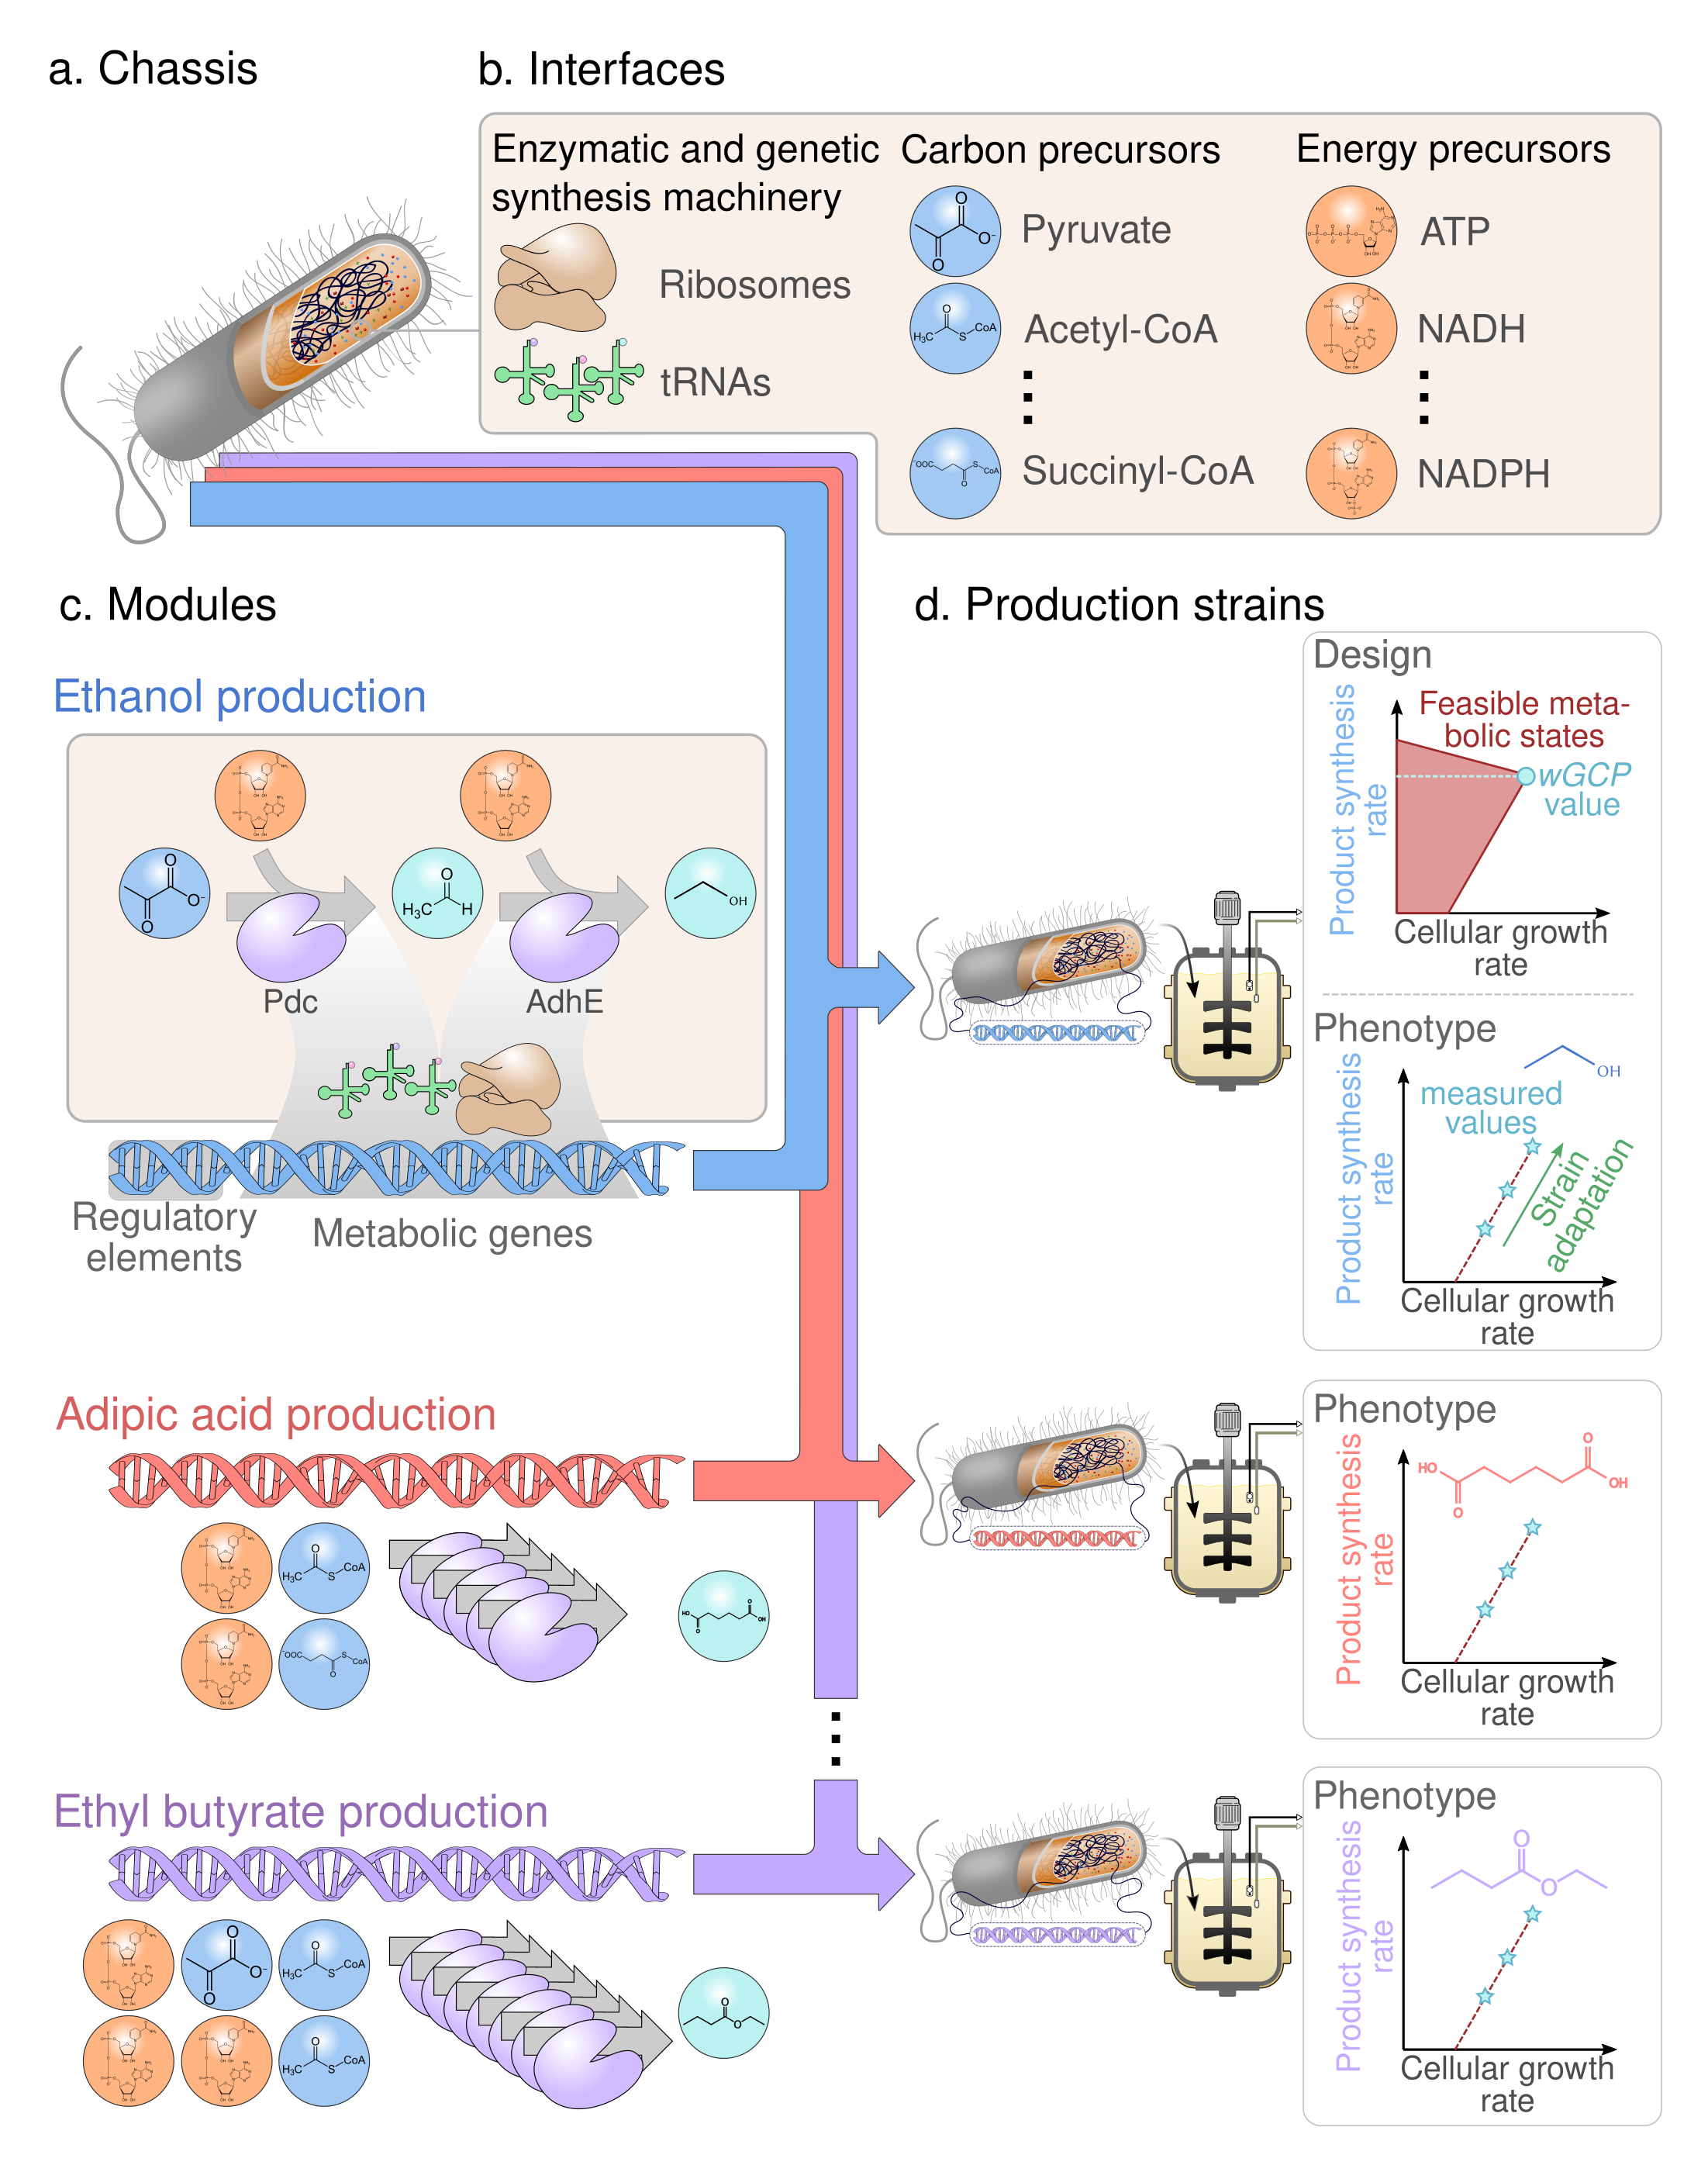
\includegraphics[width=\textwidth,height=.8\textheight,keepaspectratio]{modcell.png}
    \caption[Principles of modular cell design]{Principles of modular cell design. (a) Modular cell chassis. (b) Interfaces. (c) Production modules. (d) Production strains. A modular cell is designed to provide the necessary precursors for biosynthesis pathway modules that are independently assembled with the modular cell to generate production strains exhibiting desirable phenotypes. The \textit{wGCP} phenotype, one of the possible design objectives, enforces the coupling between the desirable product synthesis rate and the maximum cellular growth rate.}
    \label{fig5:modcell}
\end{figure}
%}

\subsubsection{Multi-objective optimization formulation}
The modular cell design problem is stated as a general multi-objective optimization problem of the form:
\begin{equation}
\underset{x}{\text{max}} \quad  F(x) = (f_{1}(x), f_{2}(x), \ldots, f_K (x))^\top  \quad  \text{s.t. } x \in X \label{eq5:multiobj}
\end{equation}
\noindent where $f_k$ is the desirable phenotype for production module $k$, $x$ are the problem variables including binary design variables corresponding to genetic manipulations, and $X$ is the set of constraints including mass balance of metabolism. Optimal solutions for the multi-objective optimization problem \eqref{eq5:multiobj} are defined using the concept of domination: A vector $a=(a_1,\dots,a_K)^\top$ \textit{dominates} another vector $b=(b_1,\dots ,b_K)^\top$, denoted as  $a\prec b$, if and only if $a_i\ge b_i \; \forall i\in\{1,2,\dots,K\}$ and $a_i\ne b_i$ for at least one $i$. A feasible solution $x^* \in X$ of the multi-objective optimization problem is called a Pareto optimal solution if and only if  there does not exist a vector $x'\in X$ such that $F(x')\prec F(x^*)$. The set of all Pareto optimal solutions is called Pareto set:
\begin{equation}
\mathit{PS}:=\{x \in X:\nexists \, x' \in X, F(x') \prec F(x)\}
\end{equation}
The projection of the Pareto set in the objective space is denoted as Pareto front:
\begin{equation}
\mathit{PF}:=\{F(x): x \in PS \}
\end{equation}
Different feasible points in $\mathit{PS}$ (i.e., different genetic manipulations) which map to a single point in $\mathit{PF}$ (i.e., the same phenotype) are denoted \textit{alternative solutions}.

The design variables $x$ in ModCell2 correspond to chassis reaction deletions, that remove undesired metabolic functions,  and module reaction insertions, that allow to identify optimal module configurations without extensive prior knowledge of the product synthesis pathway.  The constraint set $X$ is comprised of two types: (i) flux simulation constraints (e.g., mass balance,  reaction reversibility, and flux bound) that allow to predict fluxes in the design objectives upon genetic manipulations, and (ii) implementation constraints that involve the maximum number of reaction deletions in the chassis (denoted by $\alpha$) and the maximum number of module reaction insertions per module (denoted by $\beta$). The following sections describe the problem formulation in detail using the definitions compiled in the Definitions Section.

\subsubsection{Design objectives} \label{sec:do}

Design objectives, $f_k$, that correspond to specific metabolic phenotypes within the space of feasible steady-state reaction fluxes, $\Pi_{km}$, of production network $k$ (i.e., the combination of the chassis network with the production module $k$) and metabolic state $m$, are defined as follows:
\begin{alignat}{2}
		& \Pi_{km}(e_{jk}):=\{v_{jkm}\in\mathbb{R}: \\
		&	\sum_{j\in \mathcal{J}_k} S_{ijk} v_{jkm} =0  && \forall i\in \mathcal{I}_k 		\label{eq5:pi_mass_bal}\\
		& l_{jkm} e_{jk}  \le v_{jkm} \le e_{jk} u_{jkm} \;  && \forall j\in \mathcal{J}_k 			\label{eq5:pi_bound}%\\
\end{alignat}
\noindent Here, $v_{jkm}$ is the rate (mmol/gCDW/hr) of reaction $j$ in production network $k$ under metabolic state $m$.
Constraint \eqref{eq5:pi_mass_bal} enforces mass balance for all metabolites according to reaction stoichiometry given by the coefficients $S_{ijk}$, and constraint \eqref{eq5:pi_bound} imposes bounds, $l_{jkm}$ and $u_{jkm}$, for the metabolic fluxes according to reaction reversibility, experimentally measured values, and specified metabolic state.
The binary variable $e_{jk}$ is used in the overall optimization problem to indicate whether reaction $j$ in production network $k$ is removed and thus cannot carry any flux. Two metabolic states $m$ are considered, growth and non-growth, denoted $\mu$  and $\bar{\mu}$, respectively. These states are differentiated by their   flux bounds $l_{jkm}$ and $u_{jkm}$. For growth state, the lower bound of the biomass formation reaction that represents cell division, $v_{Xkm}$, is set to a minimum value of  $\gamma$, i.e., $l_{Xk\mu} = \gamma \; (\forall k \in \mathcal{K}$), while there is no upper limit to growth, i.e., $u_{Xk\mu} = \infty \; (\forall k \in \mathcal{K}$).
On the other hand, for the non-growth state both bounds are set to 0, i.e., $l_{Xk\bar{\mu}} = 0 \text{ and } u_{Xk\bar{\mu}}= 0 \; (\forall k \in \mathcal{K}$).

Given the feasible metabolic flux space, $\Pi_{km}$, the following design objectives, based on the product synthesis rate reaction, $v_{Pkm}$, are of interest:
\begin{alignat}{3}
	f_k^{wGCP} & =\frac{v_{Pk\mu}}{v_{Pk\mu}^{max}}\in[0,1], \qquad & & \forall k\in \mathcal{K} \label{eq5:obj_wgcp}\\
	f_k^{lsGCP} & =b_{\mu} \frac{v_{Pk \mu}}{v_{Pk\mu}^{max}} \, + b_{\bar{\mu}} \frac{v_{Pk \bar{\mu}}}{v_{Pk\bar{\mu}}^{max}} \in[0,b_{\mu}+b_{\bar{\mu}}], \quad  & &  \forall k\in \mathcal{K} \label{eq5:obj_lsgcp}\\
	f_k^{NGP} & = \frac{v_{Pk \bar{\mu}}}{v_{Pk\bar{\mu}}^{max}} \in[0,1], \qquad  & &  \forall k\in \mathcal{K} \label{eq5:obj_ngp}
\end{alignat}
\noindent
The product synthesis fluxes, including $v_{Pk\mu}$, $v_{Pk\mu}^{max}$, $v_{Pk\bar{\mu}}$, and $v_{Pk\bar{\mu}}^{max}$, are computed by solving the following linear programming problems:
\begin{alignat}{3}
& v_{Pk\mu} 	&\in& \,	\text{arg }	\underset{}{\text{max}} \{v_{Xk\mu}-\epsilon \, v_{Pk\mu} : v_{k\mu}\in \Pi_{k\mu}(e_{jk})	\} \label{eq5:vpgLP}	\\
& v_{P k\mu}^{max} &\in& \,	\text{arg }	\underset{}{\text{max}} \{v_{Pk \mu} : v_{k \mu} \in \Pi_{k \mu} (e_{jk} = 1, \; \forall j\in \mathcal{J}_k) 	\}   \label{eq5:vpmaxLP_g}	\\
& v_{Pk \bar{\mu}} 	&\in& \,	\text{arg }	\underset{}{\text{min}} \{v_{Pk \bar{\mu}} : v_{k \bar{\mu}} \in \Pi_{k \bar{\mu}}(e_{jk})\} \label{eq5:vpngLP} \\
& v_{Pk\bar{\mu}}^{max} &\in& \,	 \text{arg }	\underset{}{\text{max}} \{v_{Pk \bar{\mu}} : v_{k \bar{\mu}} \in \Pi_{k \bar{\mu}}(e_{jk} = 1, \; \forall j\in \mathcal{J}_k)\}  \label{eq5:vpmaxLP_ng}
\end{alignat}
\noindent
The maximum product synthesis fluxes \eqref{eq5:vpmaxLP_g} and \eqref{eq5:vpmaxLP_ng} used for objective scaling are only calculated once by not using any deleted reactions ($e_{jk}=1$), while the target phenotype fluxes \eqref{eq5:vpgLP} and \eqref{eq5:vpngLP} are functions of the deleted reactions $e_{jk}$. The design objectives, \textit{wGCP} \eqref{eq5:obj_wgcp}, \textit{lsGCP} \eqref{eq5:obj_lsgcp}, and \textit{NGP} \eqref{eq5:obj_ngp}, were previously proposed \citep{garcia2019} and briefly described here. The weak growth coupled to product formation objective (\textit{wGCP}) \eqref{eq5:obj_wgcp} seeks to maximize the minimum product rate at the maximum cellular growth, which is accomplished by a titled objective function\citep{feist2010} \eqref{eq5:vpgLP}. The linearized strong growth coupled to product formation (\textit{lsGCP}) \eqref{eq5:obj_lsgcp} objective seeks to maximize the minimum product synthesis rate at the non-growth state $v_{Pk\bar{\mu}}$ in addition to the goal of \textit{wGCP}.
In $f_k^{lsGCP}$, $b_{\mu}$, $b_{\bar{\mu}}$ are the weights on the growth  and non-growth objectives, respectively.
%In our study  $b_{\mu}=1$ and $b_{\bar{\mu}}=10$ were used to generate all results.
Finally, the non-growth production (\textit{NGP}) \eqref{eq5:obj_ngp} objective seeks to optimize the minimum product synthesis rate during the non-growth state.


\subsubsection{Design constraints} \label{sec:problem_constraints}
All the constraints of the modular cell design problem are gathered as follows:
\begin{alignat}{2}
& \mathrlap{	 \Omega:=\{f'_k \in \mathbb{R}, \, y_j, z_{jk}, d_{jk}, w_{k}, e_{jk} \in \, \{0,1\} : }\\ %
& \sum_{j\in \mathcal{C}} (1-y_j)\le \alpha 						\label{eq5:acon}\\
& \sum_{j\in \mathcal{C} - \mathcal{N}_k }z_{jk} \le \beta_k & \forall k\in \mathcal{K} 	\label{eq5:bcon}\\
& z_{jk}\le 1-y_j  & \forall j\in \mathcal{C} - \mathcal{N}_k , \;  k\in \mathcal{K}	\label{eq5:yzcon}\\
& d_{jk} = y_j \lor z_{jk} & \forall j \in \mathcal{C} ,\;  k \in \mathcal{K} \label{eq5:d_def}\\
& f'_k = f_k w_k & \forall k \in \mathcal{K} \label{eq5:fprime}\\
& e_{jk} = (d_{jk} \land w_k) \lor \lnot w_k & \forall j \in \mathcal{C} ,\;  k \in \mathcal{K} \label{eq5:e_def} \\
& w_k \le M^w f_k & \forall k \in \mathcal{K} \label{eq5:w_symmetry}\\
& v_{Pkm} \in \Psi_{km}(e_{jk})  & \forall k \in \mathcal{K} ,\;  m \in \mathcal{M} \label{eq5:psi} \, \}
\end{alignat}

\noindent Constraints \eqref{eq5:acon}-\eqref{eq5:d_def} are formulated for practical limitations and features of the modular cell. Specifically, the two variables that represent design choices for genetic manipulations include: (i) $y_j$ that takes a value of 0 if reaction $j$ is deleted in the chassis (and consequently in all production networks) and 1 otherwise and (ii) $z_{jk}$ that takes a value of 1 if reaction $j$ is inserted in production network $k$. The maximum number of reaction deletions, is limited by $\alpha$ through constraint \eqref{eq5:acon} while the maximum number of module reactions in each module $\beta_k$ is imposed by \eqref{eq5:bcon}. Constraint \eqref{eq5:bcon} excludes non-candidate reactions $\mathcal{N}_k$ (since $j\in \mathcal{C} - \mathcal{N}_k$)  so that module reactions can be fixed  (i.e., $z_{jk}=1$), according to problem-specific knowledge. Constraint \eqref{eq5:yzcon} ensures that only reactions deleted in the chassis can be inserted back to the modules.
Constraint \eqref{eq5:d_def} indicates that reaction $j$ is deleted in production network $k$ if the reaction is deleted in the chassis and not added as a module reaction. The designer can gradually increase $\alpha$ and $\beta_k$ to obtain solutions with higher performance.

Constraints \eqref{eq5:fprime}-\eqref{eq5:w_symmetry} are introduced for modeling purposes. The indicator variable, $w_k$, is introduced to allow for certain production networks to be ignored from the final solution. Without $w_k$, the whole multi-objective problem becomes infeasible if a set of deletions renders one of the production networks infeasible (e.g., its minimum growth rate cannot be accomplished). However, in practice it is acceptable for some modules not to work with the chassis cell.
If $w_k=0$, the objective value $f'_k=0$ \eqref{eq5:fprime} and reaction deletions do not apply to network $k$ since $e_{jk}=1$ \eqref{eq5:e_def}; if $w_k=1$, $f'_k = f_k$ and $e_{jk} = d_{jk}$, where $f_k$ is any of the design objectives presented earlier \eqref{eq5:obj_wgcp}-\eqref{eq5:obj_ngp}.
The use of $w_k$ is likely to introduce symmetry (i.e., alternative integer solutions with no practical meaning) due to cases where $f_k=0$ for a given $k$ while the associated production network remains feasible, allowing $w_k$ to take a value of 0 or 1. This symmetry is removed by enforcing $w_k$ to be 0 if $f_k=0$ \eqref{eq5:w_symmetry}.


Finally, constraint \eqref{eq5:psi} indicates that the fluxes featured in the design objectives, $v_{Pkm}$, are contained in the polytope $\Psi_{km}$. The space of $v_{Pkm}$ is originally defined as an optimization problem \eqref{eq5:vpgLP}-\eqref{eq5:vpmaxLP_ng}, thus representing a non-linear constraint and turning the ModCell design problem into a bilevel optimization problem. These inner optimization problems are linearized, leading to $\Psi_{km}$ as described in the following sections.

\subsubsection{Linearization of logical expressions}
The logical expressions in $\Omega$ are replaced by the following linear constraints in the final problem formulation:

\noindent $d_{jk} = y_j \lor z_{jk}$ corresponds to:
\begin{alignat}{2}
& d_{jk} \le y_j + z_{jk}  \label{eq5:d1}\\
& d_{jk} \ge y_j  \label{eq5:d2}\\
& d_{jk} \ge z_{jk} \label{eq5:d3}\\
&  0 \le d_{jk} \le 1  \label{eq5:d4}
\end{alignat}

\noindent $f'_k = f_k w_k$ corresponds to:
\begin{alignat}{2}
& f'_k \le w_k M^{obj}  \\
& f'_k \le f_k - (1-w_k) M^{obj}  \\
& f'_k \le f_k\\
& 0 \le f'_k \le M^{obj}
\end{alignat}

\noindent $e_{jk} = (d_{jk} \land w_k) \lor \lnot w_k$, given $r_{jk} = d_{jk} \land w_k$, corresponds to:
\begin{alignat}{2}
& e_{jk} = r_{jk} + 1 - w_k  \\
& r_{jk} \le w_k  \\
& r_{jk} \le d_{jk}\\
& r_{jk} \ge w_k + d_{jk} - 1 \\
& 0 \le r_{jk} \le 1
\end{alignat}

\subsubsection{Linearization of inner optimization problems} \label{sec:linearization}

Non-linear constraints expressed as linear programming problems can be linearized using basic mathematical programming theory. Consider the following canonical linear program, with primal variables $x\in\mathbb{R}^n$ and its dual variables $u\in \mathbb{R}^m$:
\begin{alignat}{3}
& \text{max} \quad \{c^\top x: Ax \le b ,\; x \ge 0 \} \label{eq5:primal} \\
& \text{min} \quad \{b^\top u: A^\top u \ge c ,\; u \ge 0 \} \label{eq5:dual}
\end{alignat}
\noindent the strong duality theorem states that the objective functions of primal (\ref{eq5:primal}) and dual (\ref{eq5:dual}) are equal at their optima, $c^\top x^* = b^\top y^*$. Thus the optimal solution to the primal problem is described by the following linear constraints:
\begin{alignat}{3}
x^* \in \{x \in \mathbb{R}^n: \\
& Ax \le b \\
& A^\top u \ge c \\
& c^\top x = b^\top u\\
& x,u \ge 0 \,\}
\end{alignat}

Using the strong duality theorem as presented by Maranas and Zomorrodi \citep{maranas2016}, the inner optimization problems \eqref{eq5:psi} are linearized as follows:
\begin{alignat}{2}
&	\Psi_{km}(e_{jk}) := \{v_{jkm} \in \mathbb{R}:  \\
%
&	\sum_{j\in \mathcal{J}_k} S_{ijk} v_{jkm} =0  && \forall i\in \mathcal{I}_k 		\label{eq5:primal_mass_bal}\\
		& l_{jkm} e_{jk}  \le v_{jkm} \le e_{jk} u_{jkm} \;  && \forall j\in \mathcal{J}_k 			\label{eq5:primal_bound}\\
&\sum_{i\in \mathcal{I}_k} \lambda_{ikm} S_{ijk}-\mu_{jkm}^{l} +\mu_{jkm}^{u}  = c_{jkm} && \forall j\in \mathcal{J}_k	\label{eq5:dual-eq}\\
%
& \lambda_{ikm} \in \mathbb{R} && \forall i \in \mathcal{I}_k \label{eq5:dual-bounds-lambda}\\
&0\le \mu_{jkm}^{l} \le M && \forall j\in \mathcal{J}_k								\label{eq5:dual-bounds-mul}	\\
&0\le \mu_{jkm}^{u} \le M && \forall j\in \mathcal{J}_k								\label{eq5:dual-bounds-muu} \\
%
\nonumber &\sum_{j\in \mathcal{J}_k} c_{jkm} v_{jkm}=
-\sum_{j\in \mathcal{J}_k - \mathcal{C}}(l_{jkm}\mu_{jkm}^{l})\, +
\sum_{j\in \mathcal{J}_k - \mathcal{C}}(u_{jkm}\mu_{jkm}^{u}) \,
\label{eq5:sd}	\\ &\phantom{{}=1}
-\sum_{j\in C}(l_{jkm}p_{jkm}^{l}) \,+
\sum_{j\in C}(u_{jkm} p_{jkm}^{u})\\
%
& p_{jkm}^{l}\le e_{jk} M && \forall j\in \mathcal{C}				\label{eq5:lin1}	\\
&\mu_{jkm}^{l}-(1-e_{jk})M \le p_{jkm}^{l} \le \mu_{jkm}^{l} && \forall j\in \mathcal{C} \label{eq5:lin2} \\
&0\le p_{jkm}^{l}\le M && \forall j\in \mathcal{C} \label{eq5:lin3}\\
%
& p_{jkm}^{u}\le e_{jk} M  && \forall j\in \mathcal{C} \label{eq5:lin4}\\
&\mu_{jkm}^{u}-(1-e_{jk}) M \le p_{jkm}^{u}\le \mu_{jkm}^{u} && \forall j\in  \mathcal{C} \label{eq5:lin5} \\
&0\le p_{jkm}^{u}\le M && \forall j\in \mathcal{C} \label{eq5:lin6}  \, \}
\end{alignat}
\noindent Constraints \eqref{eq5:primal_mass_bal}-\eqref{eq5:primal_bound} correspond to the primal metabolic network problem and were introduced earlier in $\Pi_{km}$.
Constraints \eqref{eq5:dual-eq}-\eqref{eq5:dual-bounds-muu} correspond to the dual problem. We use the dual variables, $\lambda_{ikm}$, for the primal mass balance constraints \eqref{eq5:primal_mass_bal}, together with $\mu^{l}_{jkm}$ and $\mu^{u}_{jkm}$ for the primal flux bound inequalities \eqref{eq5:primal_bound} involving lower and upper reaction bounds respectively.
Constraints \eqref{eq5:dual-bounds-lambda}-\eqref{eq5:dual-bounds-muu} emphasize the domain of the dual variables, with $M$ being a large value above the expected value of any dual variable.
Constraints \eqref{eq5:sd}-\eqref{eq5:lin6} correspond to the strong duality equality. The left hand side of the strong duality equality \eqref{eq5:sd} features the objectives presented in \eqref{eq5:vpgLP} for $m=\mu$ and \eqref{eq5:vpngLP} for $m=\bar{\mu}$. On the right hand side, products of binary and continuous variables appear, thus requiring linearization variables $p_{jkm}^l$ and $p_{jkm}^u$. Constraints \eqref{eq5:lin1}-\eqref{eq5:lin6} ensure that $p_{jkm}^l=e_{jk} \mu_{jkm}^l$ and $p_{jkm}^u = e_{jk} \mu_{jkm}^u$.

\subsubsection{Conversion of a multi-objective problem into a single-objective problem}

The multi-objective optimization problem \eqref{eq5:multiobj} is now described entirely in terms of linear constraints through $\Omega$.
However, to make the formulation compatible with MILP solver algorithms, the objective function vector, $f'$, must be expressed as a scalar. To accomplish this without loss of relevant information, we employed blended and goal attainment formulations \citep{marler2004}.

\paragraph{Blended formulation}
In the blended formulation all objectives are summed as follows:
\begin{equation}
\underset{}{\text{max}} \quad \sum_{k\in \mathcal{K}} a_k\, f'_k  \quad  \text{s.t. } f' \in \Omega \label{eq5:blended}
\end{equation}

\noindent where $a_k$ is a scalar weighting factor associated with the design objective of product $k$.  Different Pareto optimal solutions can be obtained by varying these weights. The blended formulation always provides Pareto optimal solutions as long as $a_k>0 \; (\forall k\in K$). In practice, the product priority, $a_k$, can be determined by criteria such as product market value or ``pathway readiness level" (i.e., certain pathways are easier to engineer than others).

\paragraph{Goal attainment formulation}
In the goal attainment problem a target value is defined for each objective:
\begin{alignat}{3}
& \underset{}{\text{min}}
\quad \sum_{k \in \mathcal{K}} (a_k^+ \delta_k^+ + a_k^-  \delta_k^-) \label{eq5:goal_obj} \\
\nonumber & \text{s.t. }  \qquad \\
& \qquad f'_k + \delta_k^+ - \delta_k^- = g_k & \forall k \in \mathcal{K} \label{eq5:goal_con}\\
&  \qquad \delta_k^+ , \delta_k^- \ge 0 & \forall k \in \mathcal{K} \\
& \qquad f' \in \Omega
\end{alignat}
The problem seeks to minimize the variables $\delta_k^+$ and $\delta_k^-$ that represent the deficiency and excess of the objective $f'_k$ from the target value $g_k$, respectively. Weighting parameters $a_k^+$ and $a_k^-$ correspond to different types of discrepancy to be minimized. In general, when it is important to meet the target value without exceeding it, we set $a_k^+ = a_k^- = 1$; however, when the design objective is required to be greater or equal than the target value, we set $a_k^+=1$ and $a_k^-=0$, effectively converting \eqref{eq5:goal_con} into $f'_k + \delta_k^+ \ge g_k$. Solutions to the goal attainment problem are not guaranteed to be Pareto optimal, even if all demands $g_k$ are met. To address this issue, the blended problem \eqref{eq5:blended} can be solved where the objectives are constrained to be equal or greater than the values found by solving the goal attainment problem. In practice, the goal attainment formulation corresponds to the identification of the modular cell \emph{compatible} with the largest number of modules. Here, a module $k$ is said to be \emph{compatible} if $f'_k \ge g_k$.


\subsection{Implementation}
\subsubsection{Metabolic models}
We used two parent models from which production networks were built, including: i) a core metabolic model of \textit{E. coli} \citep{trinh2015} to develop the ModCell2-MILP algorithm and compare with previous ModCell2 results \citep{garcia2019}, and ii) the iML1515 genome-scale metabolic model of \textit{E. coli}\citep{monk2017} for biosynthesis of a library of endogenous and heterologous metabolites, including 4 organic acids, 6 alcohols, and 10 esters (Figure~\ref{fig5:fig-s1}) \citep{akita2016, atsumi2008, layton2014, niu2014, rodriguez2014, shen2011, trinh2008, tseng2012, yim2011, yu2014}.
These models were configured as in the previous ModCell2 study\citep{garcia2019}, briefly: Anaerobic conditions were imposed by setting oxygen exchange fluxes to be 0, and the glucose uptake rate was constrained to be at most 10 mmol/gCDW/h. When using the genome-scale model iML1515 to simulate \emph{wGCP} designs, only the commonly observed fermentative products (acetate, CO$_2$, ethanol, formate, lactate, succinate) were allowed for secretion as described elsewhere \citep{kamp2017}.
%\afterpage{%
%\paragraph{Figure S1}
\begin{figure}[h]
    \centering
    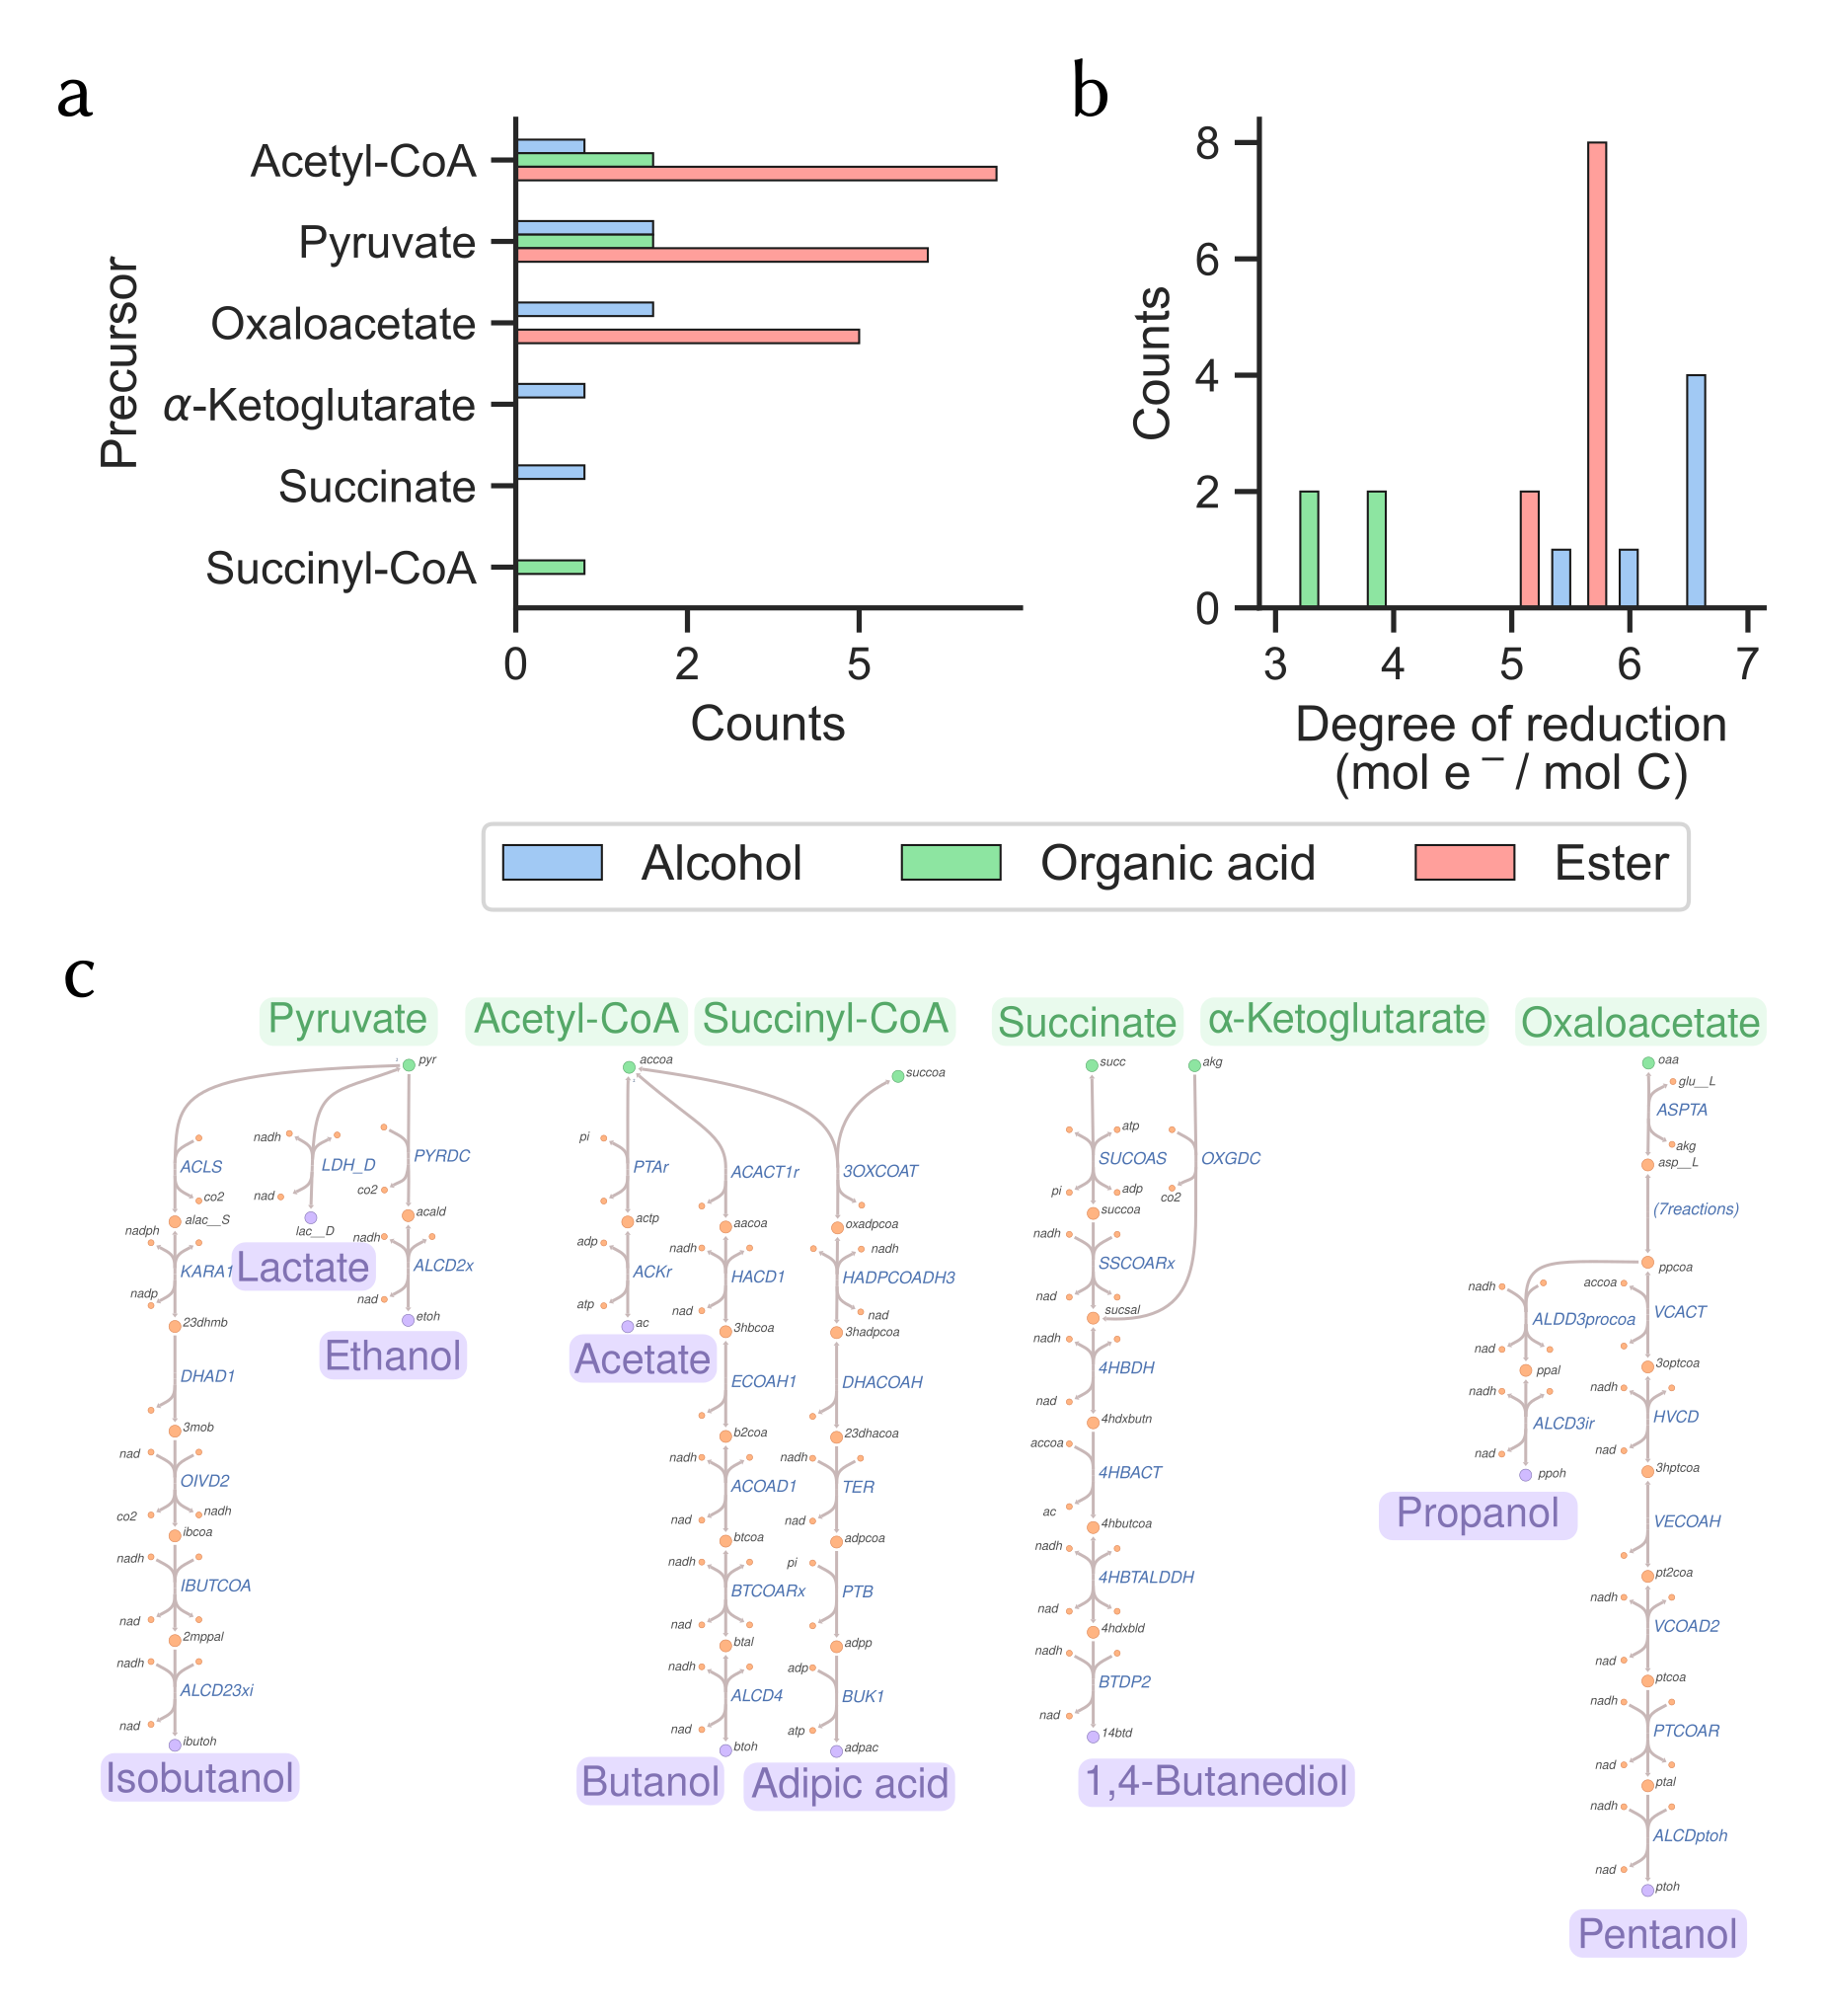
\includegraphics[width=0.7\textwidth,keepaspectratio]{Figure-S1}
    \caption[Biochemical and metabolic diversity of the 20 production modules]{
Biochemical and metabolic diversity of the 20 production modules. (a) Precursor metabolite distribution, using the 12 essential biomass precursors as a reference. (b) Degrees of reduction of the produced metabolites. (c) Production pathway metabolic modules excluding esters.
    }
    \label{fig5:fig-s1}
\end{figure}
%}

\subsubsection{ModCell2-MILP simulations}
ModCell2-MILP was implemented using Pyomo \citep{hart2017}, an algebraic modeling language embedded in the Python programming language. All simulations were performed on a computer with an Intel Core i7-3770 processor, 32 GB of random access memory, and the Arch Linux operative system. The implementation and scripts used to generate the results of this manuscript are available as part of the ModCell2 package via File S2  and \url{https://github.com/trinhlab/modcell2}.
\subsubsection{Optimization solver configuration} \label{sec:solver}
 The Pyomo \citep{hart2017} implementation of ModCell2-MILP was solved with IBM Ilog Cplex 12.8.0. To avoid incorrect solutions associated with numerical issues the following Cplex parameters were changed from their default values: (i) \textit{numerical emphasis} was set to ``true", (ii) \textit{integrality tolerance} was lowered to $10^{-7}$, and (iii) the \textit{MIP pool relative gap} was increased to $10^{-4}$ for enumerating alternative solutions.  Alternative solutions were enumerated using the Cplex ``populate" procedure.


\subsection{Analysis methods}
\subsubsection{Reference flux distribution} \label{sec:flux}
The reference flux distribution, $\frac{v_{jk}^*}{|v_{Sk}^*|}$, is determined by solving the following quadratic program based on the parsimonious enzyme usage hypothesis \citep{machado2014, lewis2010}:
\begin{alignat}{3}
    & \underset{v_{jk}}{\text{min}} \label{eq5:pfba_obj}
\quad \sum_{j \in \mathcal{J}_k} v_{jk}^2 \\
\nonumber & \text{s.t. }  \qquad \\
	& \qquad 	\sum_{j\in \mathcal{J}_k} S_{ijk} v_{jkm} =0  \quad && \forall i\in \mathcal{I}_k 		\label{eq5:pfba_mass_bal}\\
	& \qquad  l_{jk}  \le v_{jk} \le u_{jk} \;  && \forall j\in \mathcal{J}_k 			\label{eq5:pfba_bounds}\\
	& \qquad  v_{Xk} = \text{MaxDesignBio} 			\label{eq5:pfba_bio}
\end{alignat}
\noindent  Constraint \eqref{eq5:pfba_mass_bal} corresponds to mass balance for the metabolic network.
Constraint \eqref{eq5:pfba_bounds} corresponds to reaction bounds, including reaction deletions found in the modular cell design problem.
Constraint \eqref{eq5:pfba_bio} fixes the biomass formation rate, $v_{Xk}$, to the maximum reachable by the design.
This value (MaxDesignBio) is obtained by maximizing $v_{Xk}$ subject to \eqref{eq5:pfba_mass_bal} and \eqref{eq5:pfba_bounds}.
The reference flux distribution $\frac{v_{jk}^*}{|v_{Sk}^*|}$ represents the desired metabolic state of a \textit{wGCP} designed production network. This distribution, if feasible, is unique because the convex optimization problem is formulated with a positive definite quadratic objective function (see Theorem 16.4 in Nocedal and Wright\citep{nocedal2006}). % This is not hard to show here given that the objective function is strictly convex. However, showing the strict convexity requires multivariate calculus (taylors series or frechet derivatives) which are very likely to loose our audience.


\subsubsection{Flux variance clustering}

Flux variance clustering (FVC) seeks to identify and group reactions that exhibit high flux changes under different conditions. Reactions with high flux variance can be considered as metabolic interfaces between core metabolic processes and pathway modules. In our study, each condition corresponds to a different product synthesis phenotype.  FVC implementation entails three steps. First, flux distributions are simulated for each condition and standard deviations for each reaction are calculated. Then, a standard deviation threshold is set to select the reactions with highest flux changes across conditions. Finally, these selected reactions are clustered to identify patterns that repeat under specific conditions. The filtering threshold is set to capture the top reactions with most change while maintaining a sufficiently small list that is biologically meaningful. In our study, we chose an \emph{ad-hoc} value that captures well-known reactions in \textit{E. coli} central metabolism. To cluster the selected reactions, only flux magnitudes, not directionality, were considered in our study. Further, each reaction flux was normalized by the maximum value of that same reaction across all production networks. Clustering was performed using the method \emph{clustermap()} with default clustering-related parameters from the Python library Seaborn 0.9.
%In principle, pathway ontology enrichment or biochemical connectivity of the resulting clusters can potentially be used as metrics to systematically identify a threshold but not explored here.


\subsubsection{Flux sampling} \label{sec:sampling}
To determine an ensemble of flux distributions for a production network, we used the ACHR algorithm \citep{kaufman1998} in the COBRA toolbox \citep{heirendt2017}. Constraints for flux sampling simulation include the reaction deletions and module reactions found in the ModCell design problem solution, a fixed substrate uptake rate of -10 mmol glucose/gCDW/hr, and a minimum product synthesis flux of 50\% of its maximum value.

\subsubsection{Metabolic map drawing}
Drawings of metabolic map were performed using the Escher \citep{king2015a} tool (\url{https://escher.github.io}) that produces \textit{svg} files. Coloring, highlighting candidate reactions, and other systematic adjustments of metabolic maps were done with the Python-based \textit{lxml} module. Additional editing for visual enhancement was done with the Inkscape software.



\section{Results and discussion}

\subsection{Performance and solution time optimization of ModCell2-MILP}
\subsubsection{ModCell2-MILP can not only reproduce the results of the original ModCell2 formulation but also find more alternative solutions}
To evaluate ModCell2-MILP, we compared its performance with the previously developed ModCell2 platform\citep{garcia2019} that solves the optimization problem with multi-objective evolutionary algorithms (MOEAs). As a basis of comparison, we used the same \textit{E. coli} core metabolic model, maximum number of deletion reactions $\alpha$, and maximum number of module-specific reactions $\beta_k$ for both ModCell2 and ModCell2-MILP. Due to fundamental differences in problem formulations for MOEA and MILP, we used the \textit{lsGCP} design objective for ModCell2-MILP with multiple weighting factors, $a_k$, specifically selected to reproduce previous results, in the blended formulation and the \textit{sGCP} design objective for ModCell2 (File S1). The results showed that ModCell2-MILP could generate the same Pareto optimal designs like ModCell2. In addition, ModCell2-MILP enumerated a larger number of alternative solutions than ModCell2. For example, the design named \textit{sGCP-5-0-6} generated by ModCell2 had 3 alternative solutions while ModCell2-MILP found 8 alternative solutions. By increasing $\alpha$ to 8 and $\beta$ to 2, we could identify a utopia design (i.e., one solution with the maximum value for all objectives) with 192 alternative solutions, expanding the possibilities for experimental implementation.


\subsubsection{Tuning MILP formulations significantly improves solution times}
We considered three techniques that can improve solution times of ModCell2-MILP, including:

(i) \textit{Fixing the network feasibility indicator} $w_k$. If all modules are expected to be compatible with a final ModCell design (i.e., $f_k > 0,\, \forall k \in \mathcal{K}$), $w_k$ is set to be 1 for all $k \in \mathcal{K}$ to avoid computational efforts in finding non-optimal feasible solutions.

(ii) \textit{Flux bound tightening}. Constraints of the form $ e_{jkm} l_{jkm} \le v_{jkm} \le e_{jkm} u_{jkm}$ are known to result in weak linear relaxations, i.e., feasible values of $v_{jkm}$ are far from their bounds $l_{jkm}$ and $u_{jkm}$. To tighten the formulation by making continuous relaxations closer to the feasible integer solution, smaller values of $u_{jkm}$ and $l_{jkm}$ are determined by solving a series of linear programs that maximize and minimize each flux $v_{jkm}$ in the parent production networks $\Pi_{km}(e_{jk}=1, \, \forall j \in \mathcal{J}_k)$.

(iii) \textit{Benders decomposition}. ModCell2-MILP has a separable structure compatible with Benders decomposition\citep{geoffrion1972, fischetti2016} that creates a  master problem, using binary variables and associated constraints \eqref{eq5:acon}-\eqref{eq5:w_symmetry}, and sub-problems for each production network $\Psi_{km}(e_{jk})$ with fixed binary variables. This decomposition implementation is automatically done by Cplex 12.8.

We evaluated these three techniques for tuning MILP formulations and used the core\textit{ E. coli} model\citep{garcia2019} for the benchmark study. The results showed that flux bound tightening, fixed $w_k$, and Benders decomposition could reduce the solution time to find solutions by 50\%, 80\%, and  95\%, respectively (Table~\ref{tab5:timing}). By combining these techniques, the solution time was shortened by 96\% from 63.3 s to 2.8 s. In subsequent studies, we used these three tuning techniques to solve the ModCell design problem unless otherwise noted.

%\begin{table}[!ht]
\begin{table}[ht]
    \caption[Solution time reduction by tuning the ModCell2-MILP formulation]{Solution time reduction by tuning the ModCell2-MILP formulation.
    Fixed network indicator means $w_k = 1\;, \forall k \in \mathcal{K}$. The simulations were performed in triplicates.
    }
    \centering
	%Table: Solution times (n=3) for \alpha=5 and \beta=1 and objective lsGCP.
\rowcolors{2}{gray!25}{white}
\begin{tabular}{cccc}    \toprule
	\multicolumn{1}{>{\centering\arraybackslash}m{20mm}}{Feasibility indicator $w_k$  fixed} &
	\multicolumn{1}{>{\centering\arraybackslash}m{20mm}}{Benders decomposition} &
	\multicolumn{1}{>{\centering\arraybackslash}m{20mm}}{Bounds tightened} &
	\multicolumn{1}{>{\centering\arraybackslash}m{20mm}}{Solution time (s)} \\
	\midrule
	No&No&No&63.3 $\pm$ 16.9 \\
	No&No&Yes&32.5 $\pm$ 10.2 \\
	No&Yes&No&3.6 $\pm$ 0.1 \\
	No&Yes&Yes&3.4 $\pm$ 0.4 \\
	Yes&No&No&13.8 $\pm$ 2.7 \\
	Yes&No&Yes&11.9 $\pm$ 1.7 \\
	Yes&Yes&No&2.7 $\pm$ 0.3 \\
	Yes&Yes&Yes&2.8 $\pm$ 0.1 \\
 \hline
\end{tabular}



    \label{tab5:timing}
\end{table}

\subsubsection{Choice of design parameters affect solution time}
In designing a modular cell with ModCell2-MILP, the designer needs to specify the formulation type (i.e., blended or goal attainment formulation), the target phenotype (e.g., \textit{wGCP, lsGCP}, and \textit{NGP}), and the limits of deletion reactions ($\alpha$) and module-specific reactions ($\beta_{k}$). We evaluated the impact of these parameters on solution time using the \textit{E. coli} core model (Figure~\ref{fig5:times}).  Regardless of the formulation type, increasing $\alpha$ and $\beta$ led to harder problems and hence required more solution time due to the exponentially increasing number of feasible solutions as expected. The goal attainment formulation took longer time to solve for the \textit{lsGCP} and \textit{NGP} design objectives, but about the same time for the \textit{wGCP} design objective. Interestingly, the overall difficulty of \textit{wGCP} is higher than that of \textit{lsGCP} in both the blended and goal attainment formulations, despite \textit{lsGCP} having approximately twice the number of constraints. Furthermore, the \textit{NGP} design objective could be solved most quickly, likely due to the narrower design space associated with the no-growth associated production of target metabolites.

%\afterpage{%
\begin{figure}[hp]
    \centering
    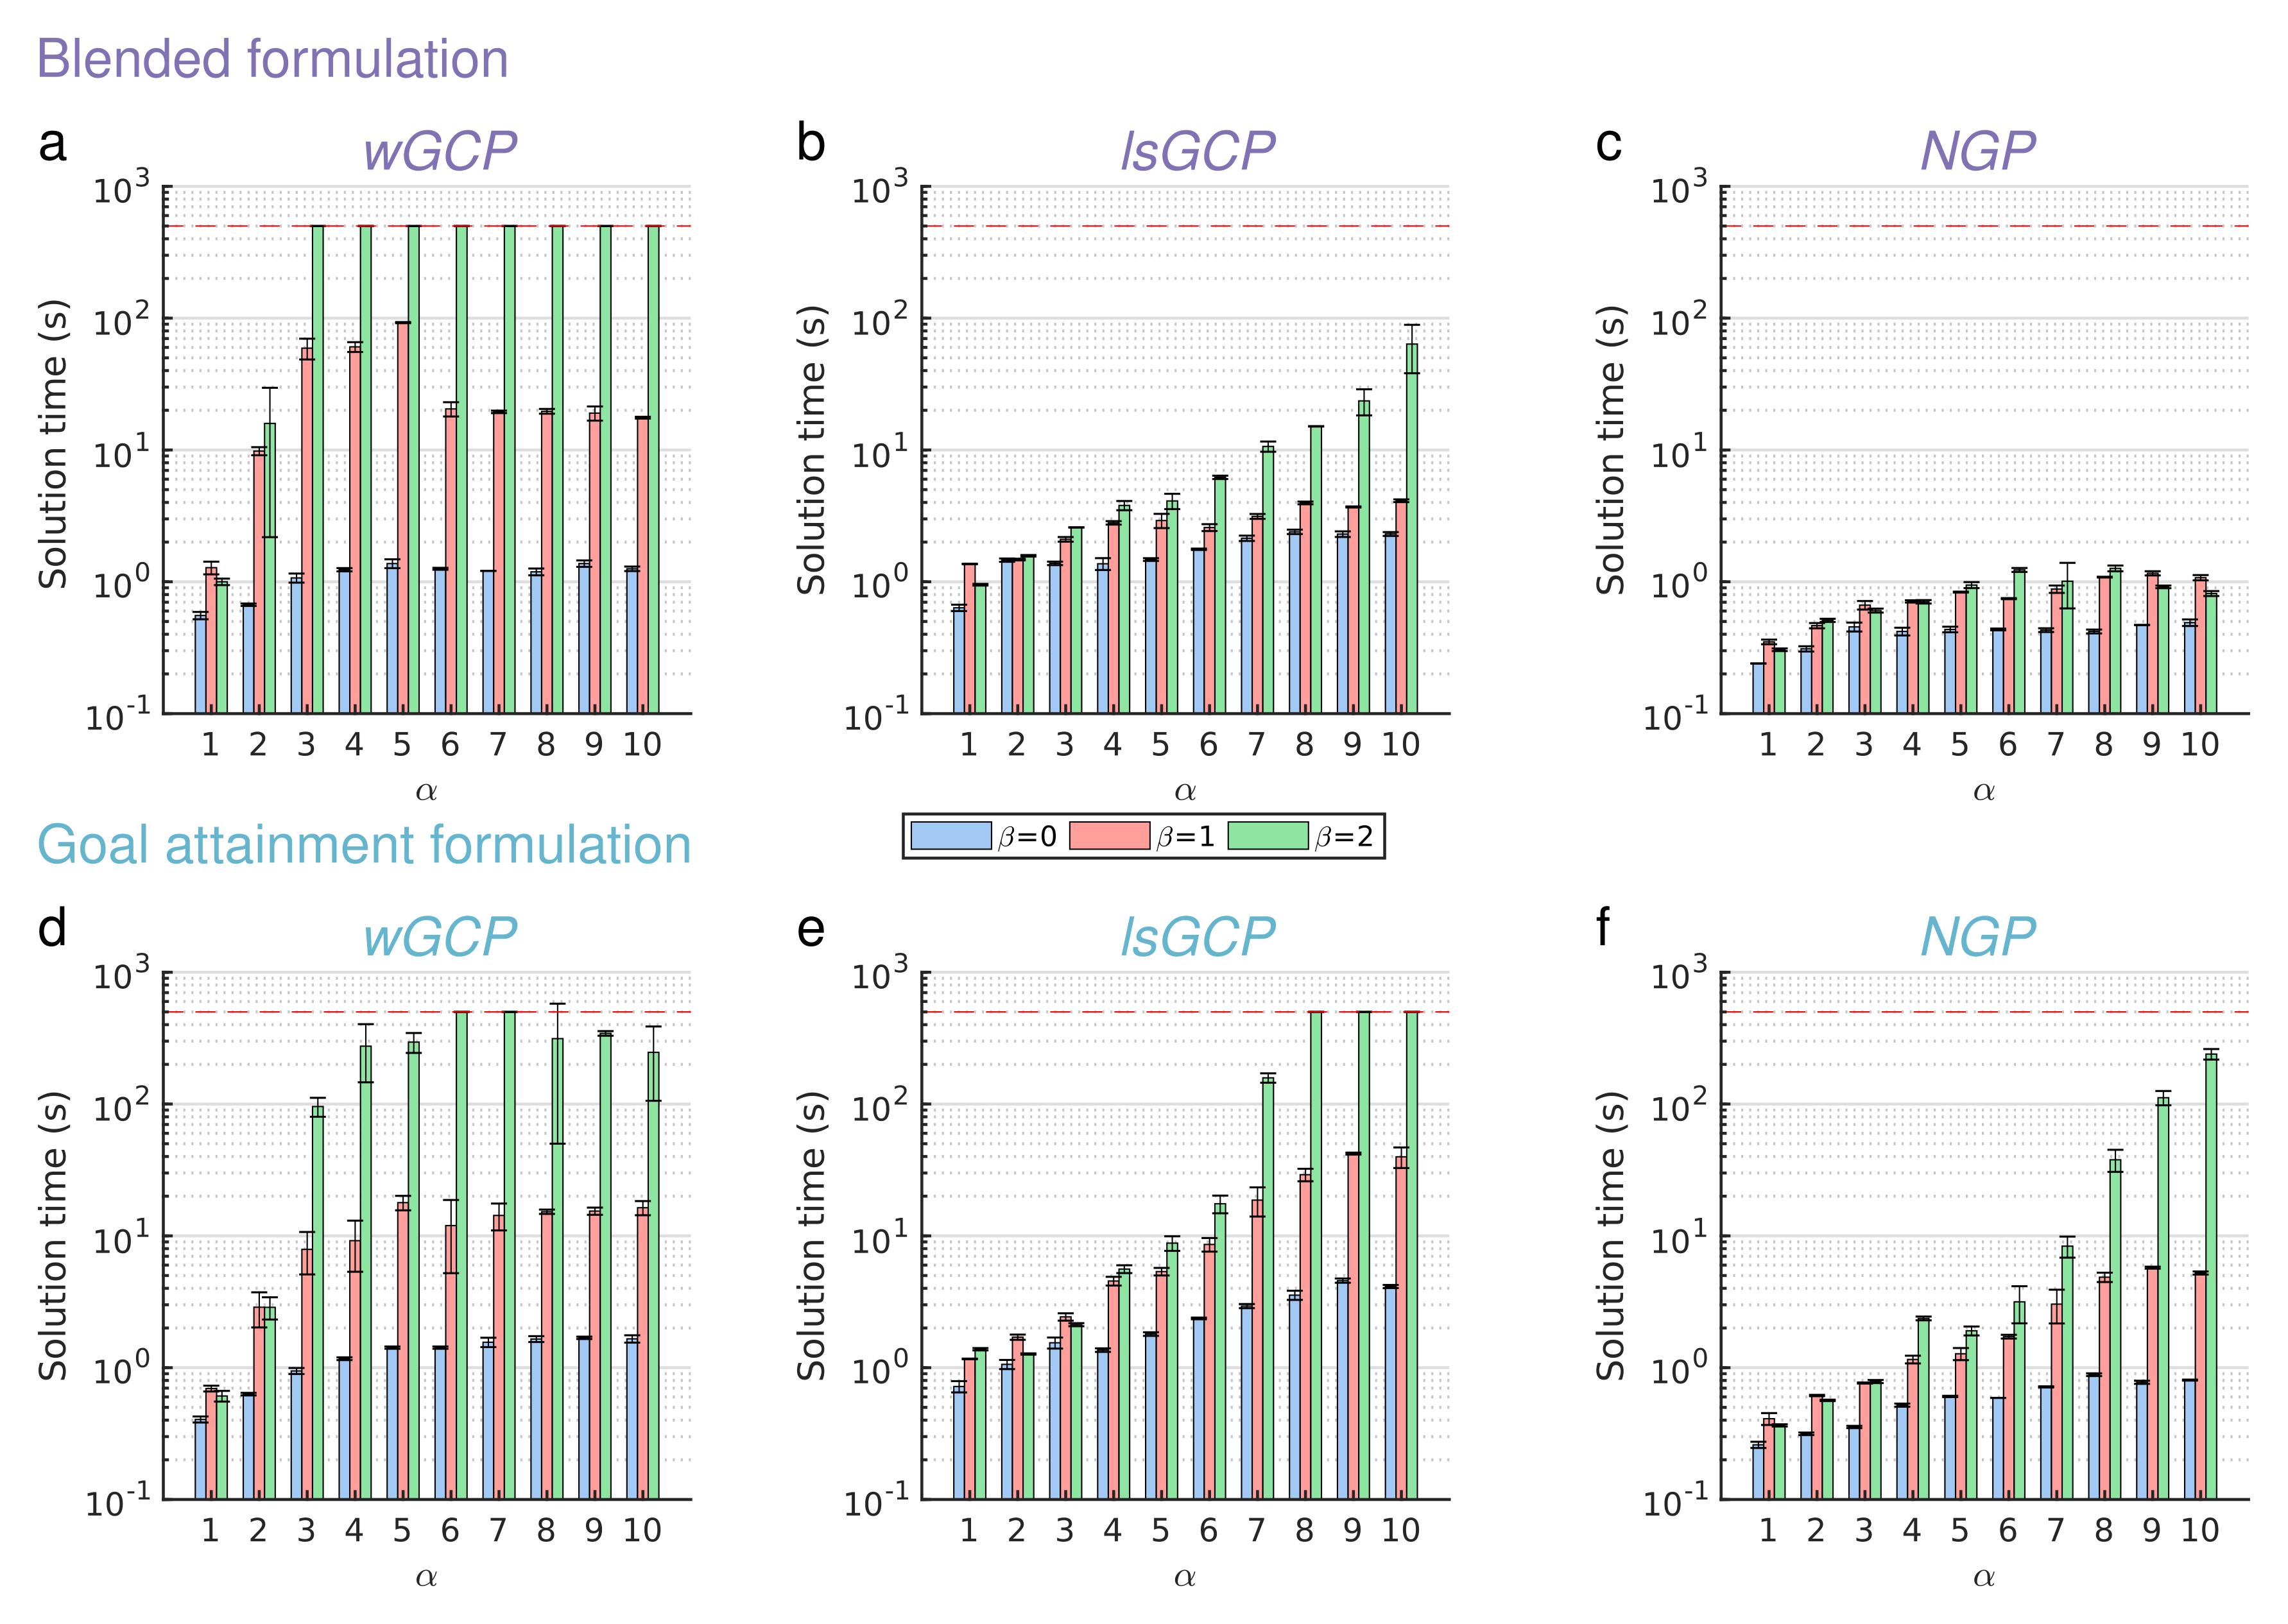
\includegraphics[width=\textwidth,height=\textheight,keepaspectratio]{performance-timing.png}
    \caption[Effect of design parameters on solution time]{Effect of design parameters on solution time. We examined the target design objective (i.e., \textit{wGCP}, \textit{lsGCP}, and \textit{NGP}) and the limits of deletion reactions $\alpha$ and endogenous module-specific reactions $\beta_k$, on computation time for solving the ModCell2-MILP problem with the blended (a-c) and goal attainment (d-f) formulations. A time limit of 500 seconds indicated by a red dashed line was used in all cases, but only reached by certain \textit{wGCP} and \textit{lsGCP} cases with $\beta \ge2$. The simulations were performed in duplicates.}
    \label{fig5:times}
\end{figure}
%}

\subsection{Design of a universal modular cell for a genome-scale metabolic model of \textit{E. coli}} \label{sec:univ_design}

\subsubsection{Reduction of the candidate reaction deletion set enables ModCell2-MILP to find modular cell designs for a large-scale metabolic network}

Finding genetic modifications towards a desired phenotype using mathematical optimization for large-scale metabolic networks is a computationally expensive task, due to the combinatorial search space spanned by a large number of reaction deletion candidates in the network \citep{feist2010, kamp2014}.
Preprocessing of metabolic networks to reduce reaction candidates is not only critical but also practical for experimental implementation. The set of reaction candidates in the iML1515 \textit{E. coli} model\citep{monk2017} was reduced from 2,712 to 276 by ModCell2 \citep{garcia2019}. Using this model and the \textit{wGCP} objective, an \textit{E.~coli} modular cell was then identified to be compatible with 17 out of 20 products with requirement of only 4 reaction deletions \citep{garcia2019}.
Since MOEA implemented in ModCell2 does not guarantee optimality, here we aimed to evaluate the capability of ModCell2-MILP for handling a large-scale metabolic network and identifying the Pareto optimality and potential alternative solutions.

We applied ModCell2-MILP to analyze the same iML1515 model with a set of 20 products using the same design parameters (i.e., $\alpha$ and $\beta_k$) and the blended formulation with all objective weights $a_k=1$. The simulation shows that ModCell2-MILP could not solve the ModCell design problem to optimality over 2 days of run time, likely due to the large number of candidate deletion reactions still present in the genome-scale model. Currently the best MILP solution algorithms do not scale well with parallel computing. In order to obtain solutions within an acceptable time, the set of candidate reactions must be further reduced. Since only a small subset of all metabolic reactions in genome-scale models tend to be deleted by strain design algorithms \citep{feist2010, king2017, garcia2019}, we used a pool of \textit{wGCP} designs with $\alpha= 4,5,6$ and $\beta = 0,1$ reported with ModCell2 \citep{garcia2019} to identify relevant deletion candidates. From a set of 601 designs found by ModCell2, only 33 out of 276 reaction deletion candidates were used at least once. Hence, these 33 reactions were used to create a new, computationally-tractable set of reaction candidates. This new set contains reactions mostly from the well-characterized central metabolic pathways (Figure~\ref{fig5:candidate-reactions}a) while the original set includes reactions in peripheral pathways that lead to biomass synthesis. Interestingly, within these 33 reaction candidates, only a few are used in most designs (Figure~\ref{fig5:candidate-reactions}b), highlighting the importance of their removal in growth-coupled production phenotypes. Reactions with high deletion frequencies mainly occur in high-flux central metabolic pathways (Figure~\ref{fig5:candidate-reactions}c), closely associated with cellular energetics and carbon precursors that interface with the production modules (Figure~\ref{fig5:candidate-reactions}d).

\begin{figure}[p]
    %\textit{Figure on previous page.}}
    \centering
    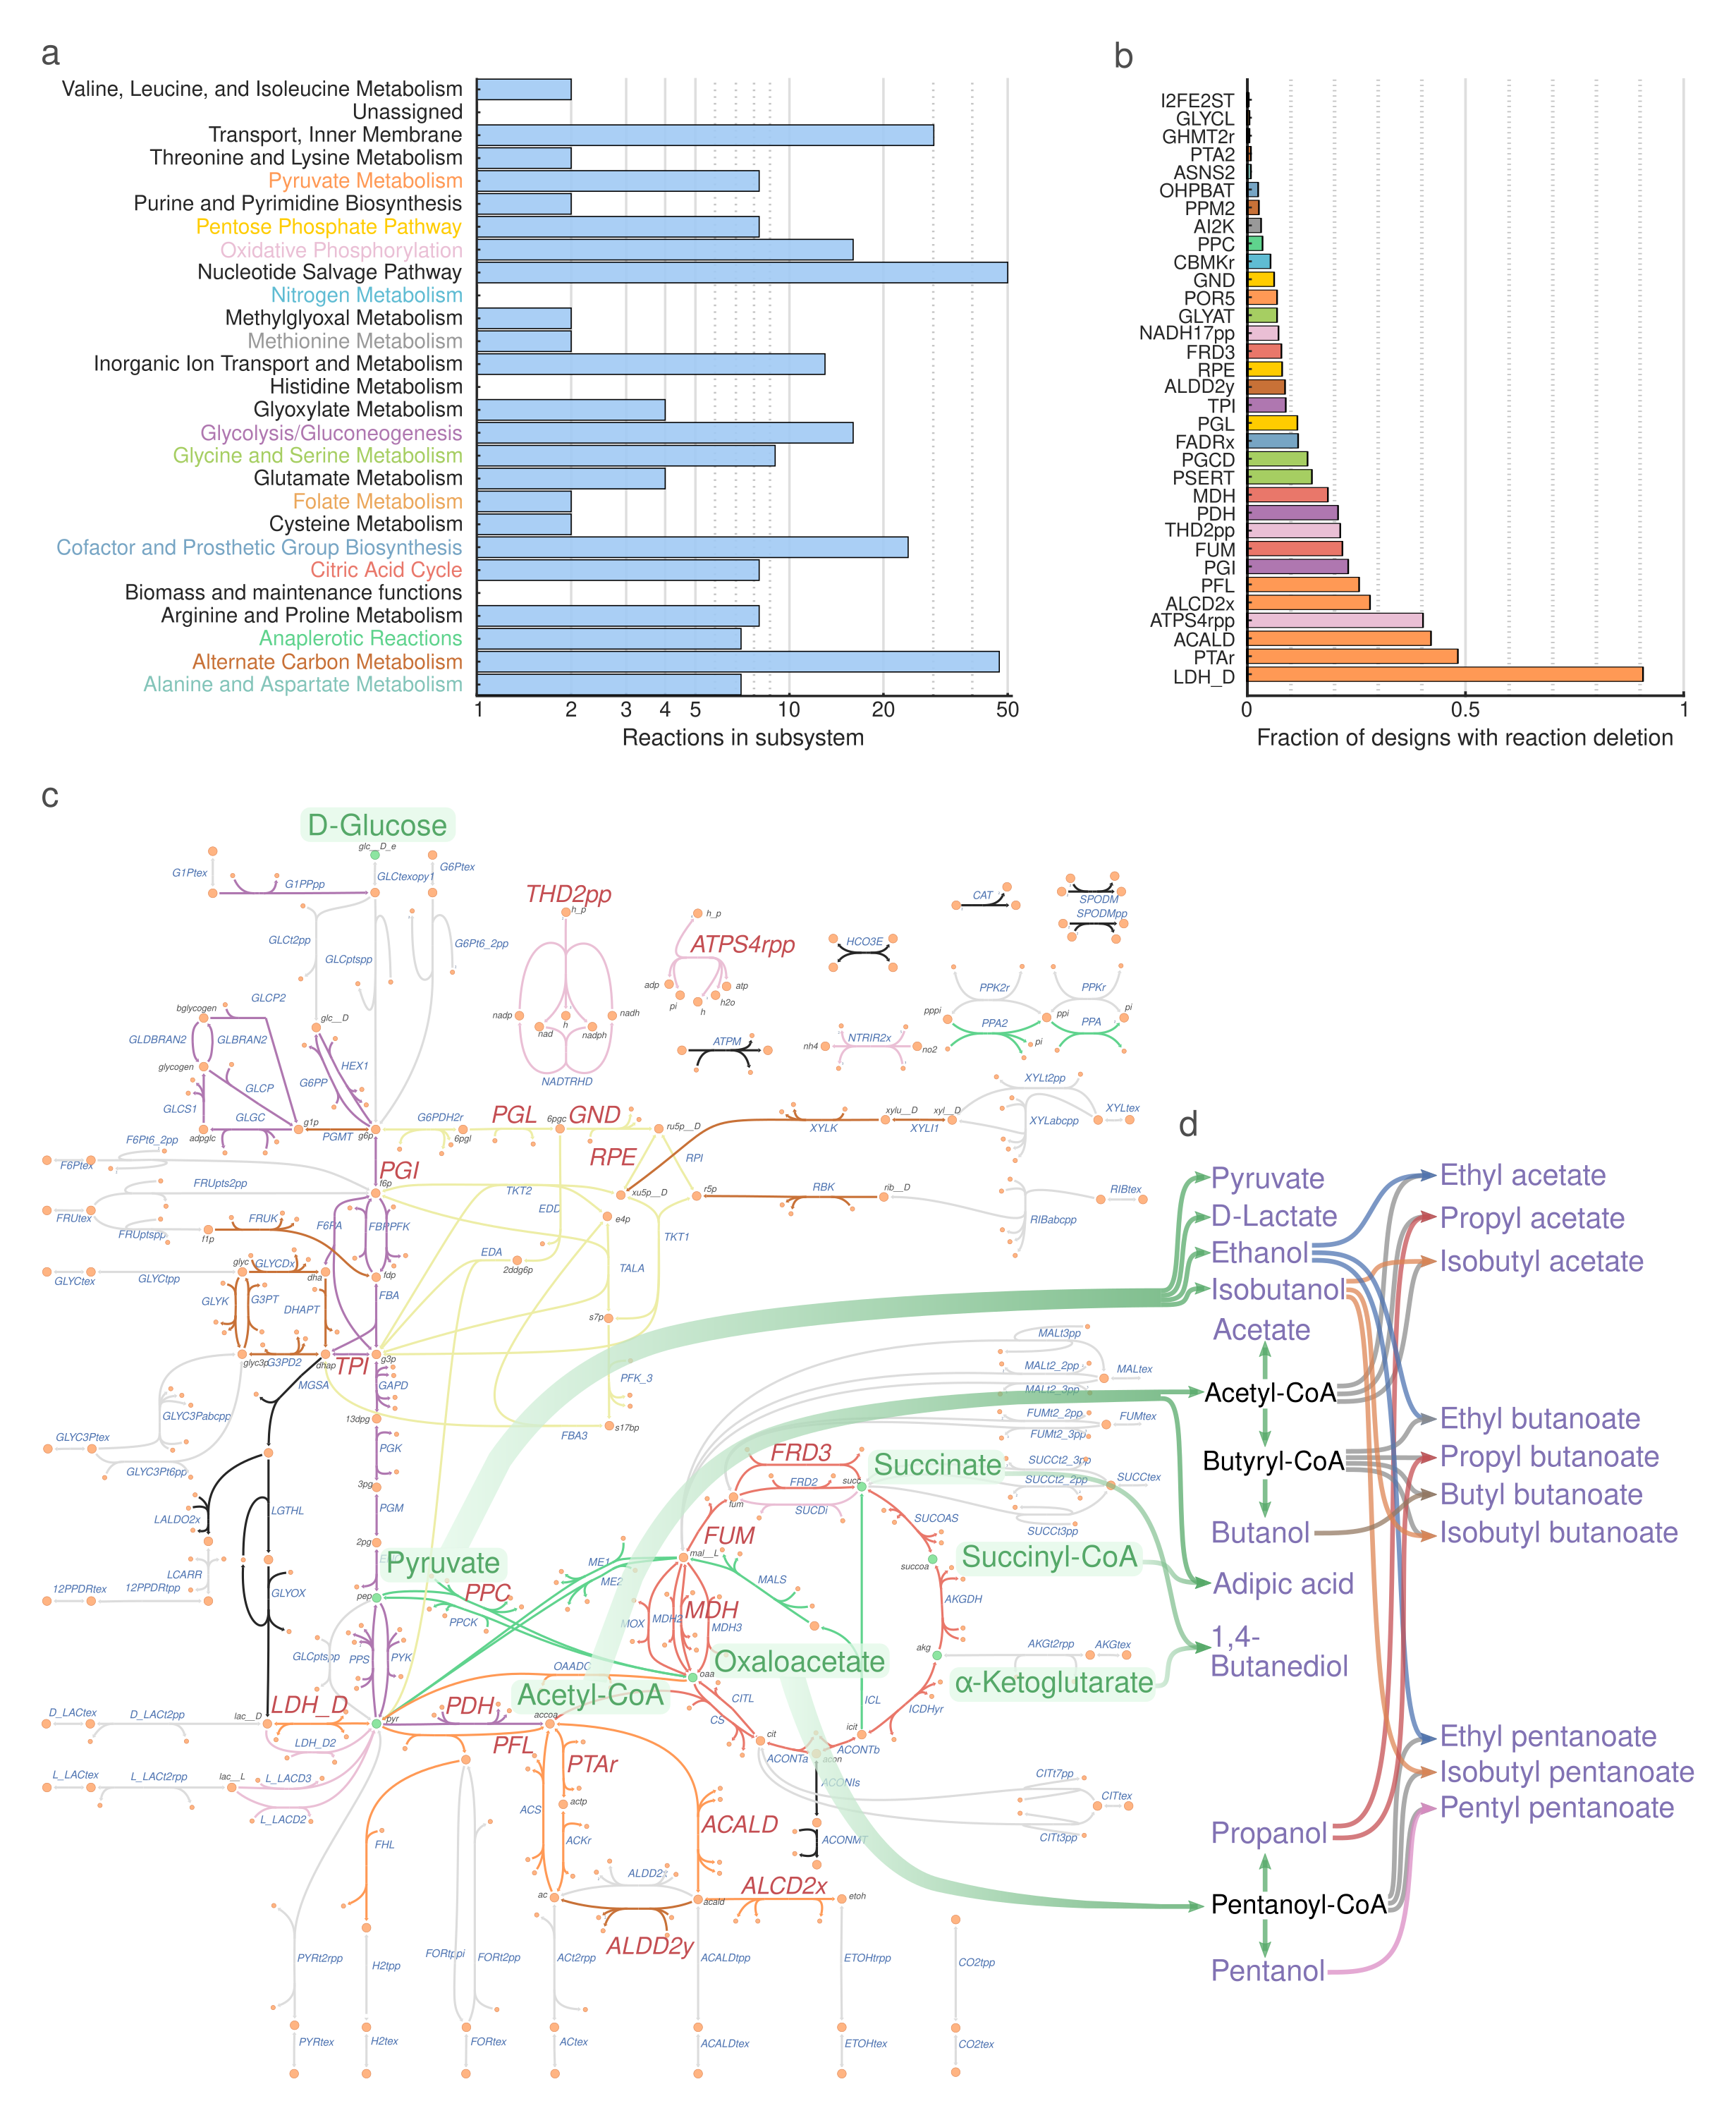
\includegraphics[height=.71\textheight,keepaspectratio]{candidate-reactions.png}
    \caption[Metabolic functions of deletion candidate reactions]{Metabolic functions of deletion candidate reactions. (a) Subsystem distribution for the original set of 276 candidate reactions in the iML1515 model. Those subsystems that contain a reaction used in at least one design are colored.  (b) Deletion frequency for the reduced set of 33 candidate reactions. The analysis is based on a pool of 601 \textit{wGCP} designs from different $\alpha$ and $\beta$ parameters whose Pareto fronts were previously determined with ModCell2.\citep{garcia2019} Bar colors indicate membership of these reactions to the subsystems. (c) Metabolic map of core metabolism. Key metabolites, including precursors for the 20 product modules (i.e., pyruvate, acetyl-CoA, succinyl-CoA, succinate, and $\alpha$-ketoglutarate), are highlighted in green. Reactions are colored according to subsytem labels indicated in (a), reactions colored in light gray do not appear  in any of the subsytems of (a), and reactions that are candidates for deletion, listed in (b), are labeled in red. (d) Link between major precursors and target products where colors are only used to facilitate visualization. Reaction and metabolite abbreviations correspond to BiGG\citep{king2015} identifiers (\protect\url{http://bigg.ucsd.edu/}).
    }
    \label{fig5:candidate-reactions}
\end{figure}
%\addtocounter{figure}{-1}
%\afterpage{%
%\begin{figure}[H]
    %\caption{\textit{Caption on next page.}}
	%\centering
    %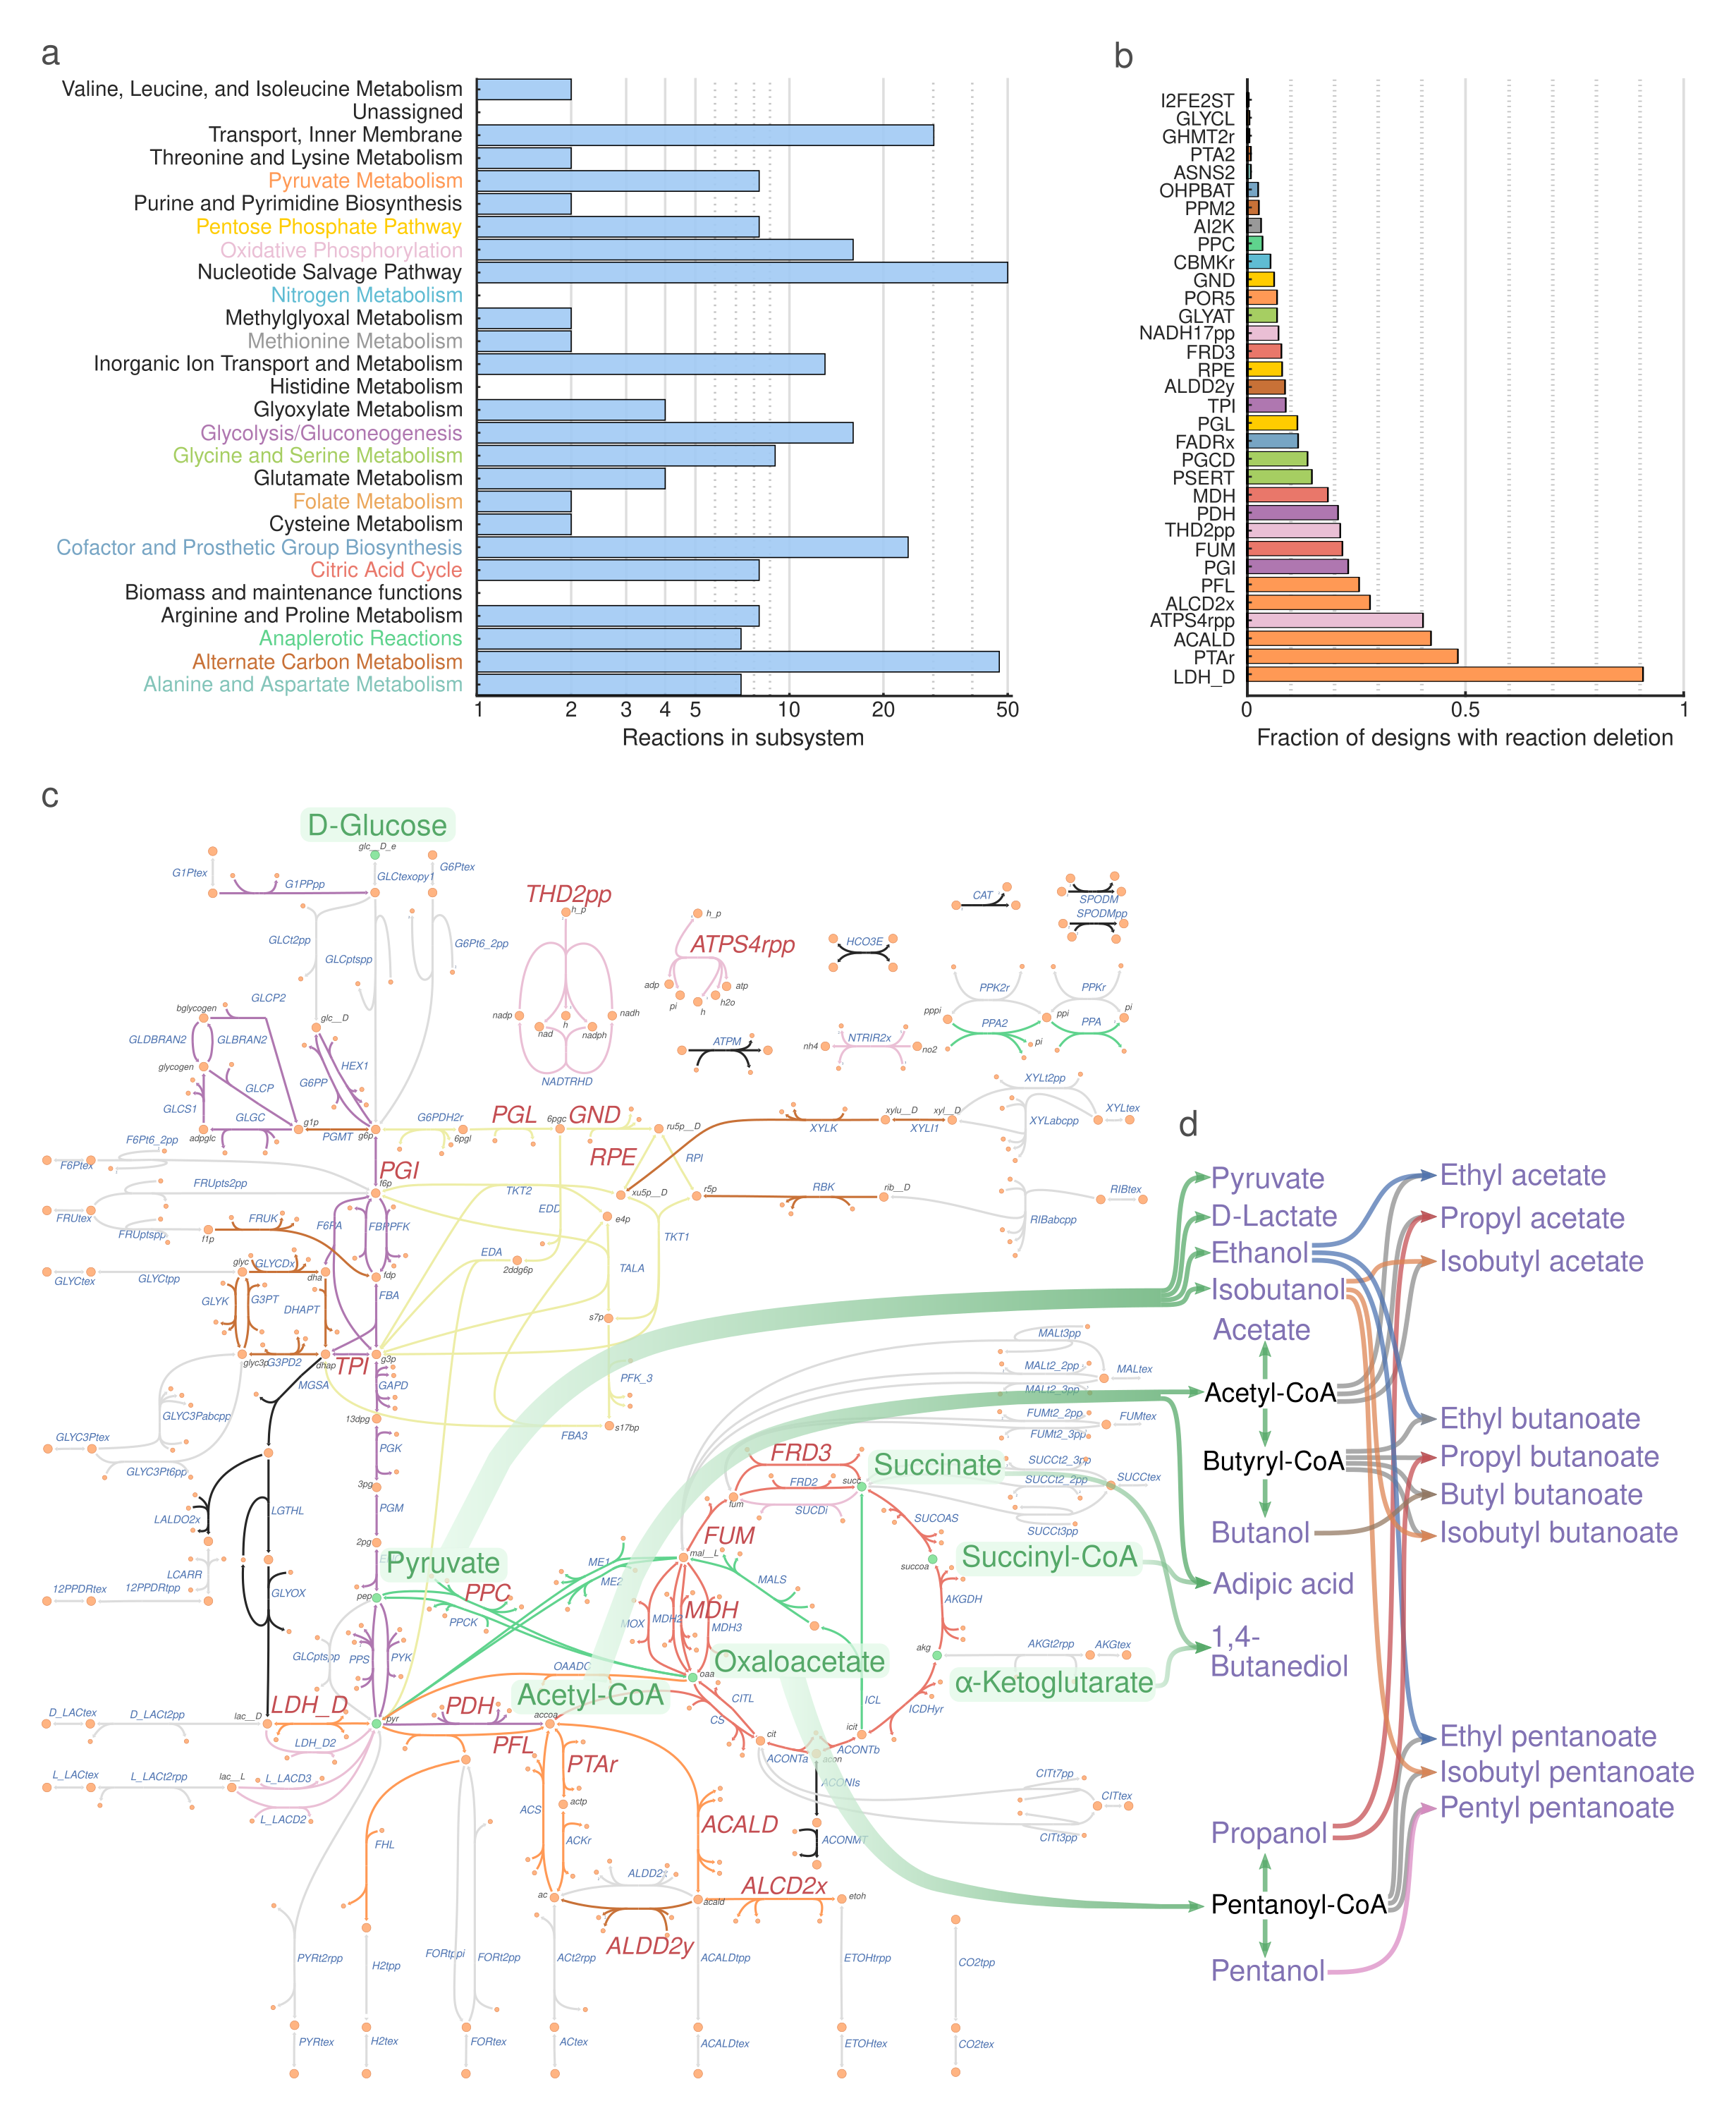
\includegraphics[height=\textheight,keepaspectratio]{candidate-reactions.png}
%\end{figure}}

Using the reduced reaction deletion candidate set, ModCell2-MILP could find an optimal solution in $\sim 30$ min and enumerated all optimal solutions in $\sim 8$ hours. All the optimal solutions found by ModCell2-MILP in this case were in agreement with those previously found by ModCell2 \citep{garcia2019}. It should be noted that a reduced deletion candidate set can be identified for any metabolic model and target products by using previous designs identified with either ModCell2 or single-phenotype strain design algorithms \citep{long2015}. This heuristic for reaction deletion candidate selection might affect design optimality to the extent that it omits relevant reactions. However, using a sufficiently informative pool of designs from other strain design algorithms helps minimize the chances of missing relevant candidates.


\subsubsection{ModCell2-MILP can identify a universal modular cell compatible with all exchangeable production modules} \label{sec:universal_design}
Based on the computationally tractable reaction deletion candidate set, we next evaluated whether the goal programming formulation could help identify a universal ModCell design that is compatible with all modules.
By screening for increasing $\alpha$ and $\beta_k$, we found that a design with $\alpha=6$ and $\beta_k=1$ could overcome the performance trade-offs between modules and hence constitute a universal modular cell that is compatible with all production networks considered (Figure~\ref{fig5:universal-design}a). Once coupled with a module, each resulting production strain displays the engineered phenotype with the defined minimum objective goal of 0.5 (i.e., 50\% of the theoretical maximum product yield attained at the maximum growth rate).
Remarkably, most products surpassed this minimum goal with yields above 90\% of the theoretical maximum values (Figure~\ref{fig5:universal-design}b). All production networks displayed a feasible metabolic space where an increase in product synthesis rate is needed to attain faster growth rates (Figure~\ref{fig5:universal-design}c). This designed phenotype is useful for optimal pathway selection using adaptive laboratory evolution \citep{fong2005, trinh2009b} and/or pathway libraries \citep{garst2017}.

%\afterpage{%
\begin{figure}[p]
%\begin{adjustwidth}{-2.25in}{0in}
    \centering
    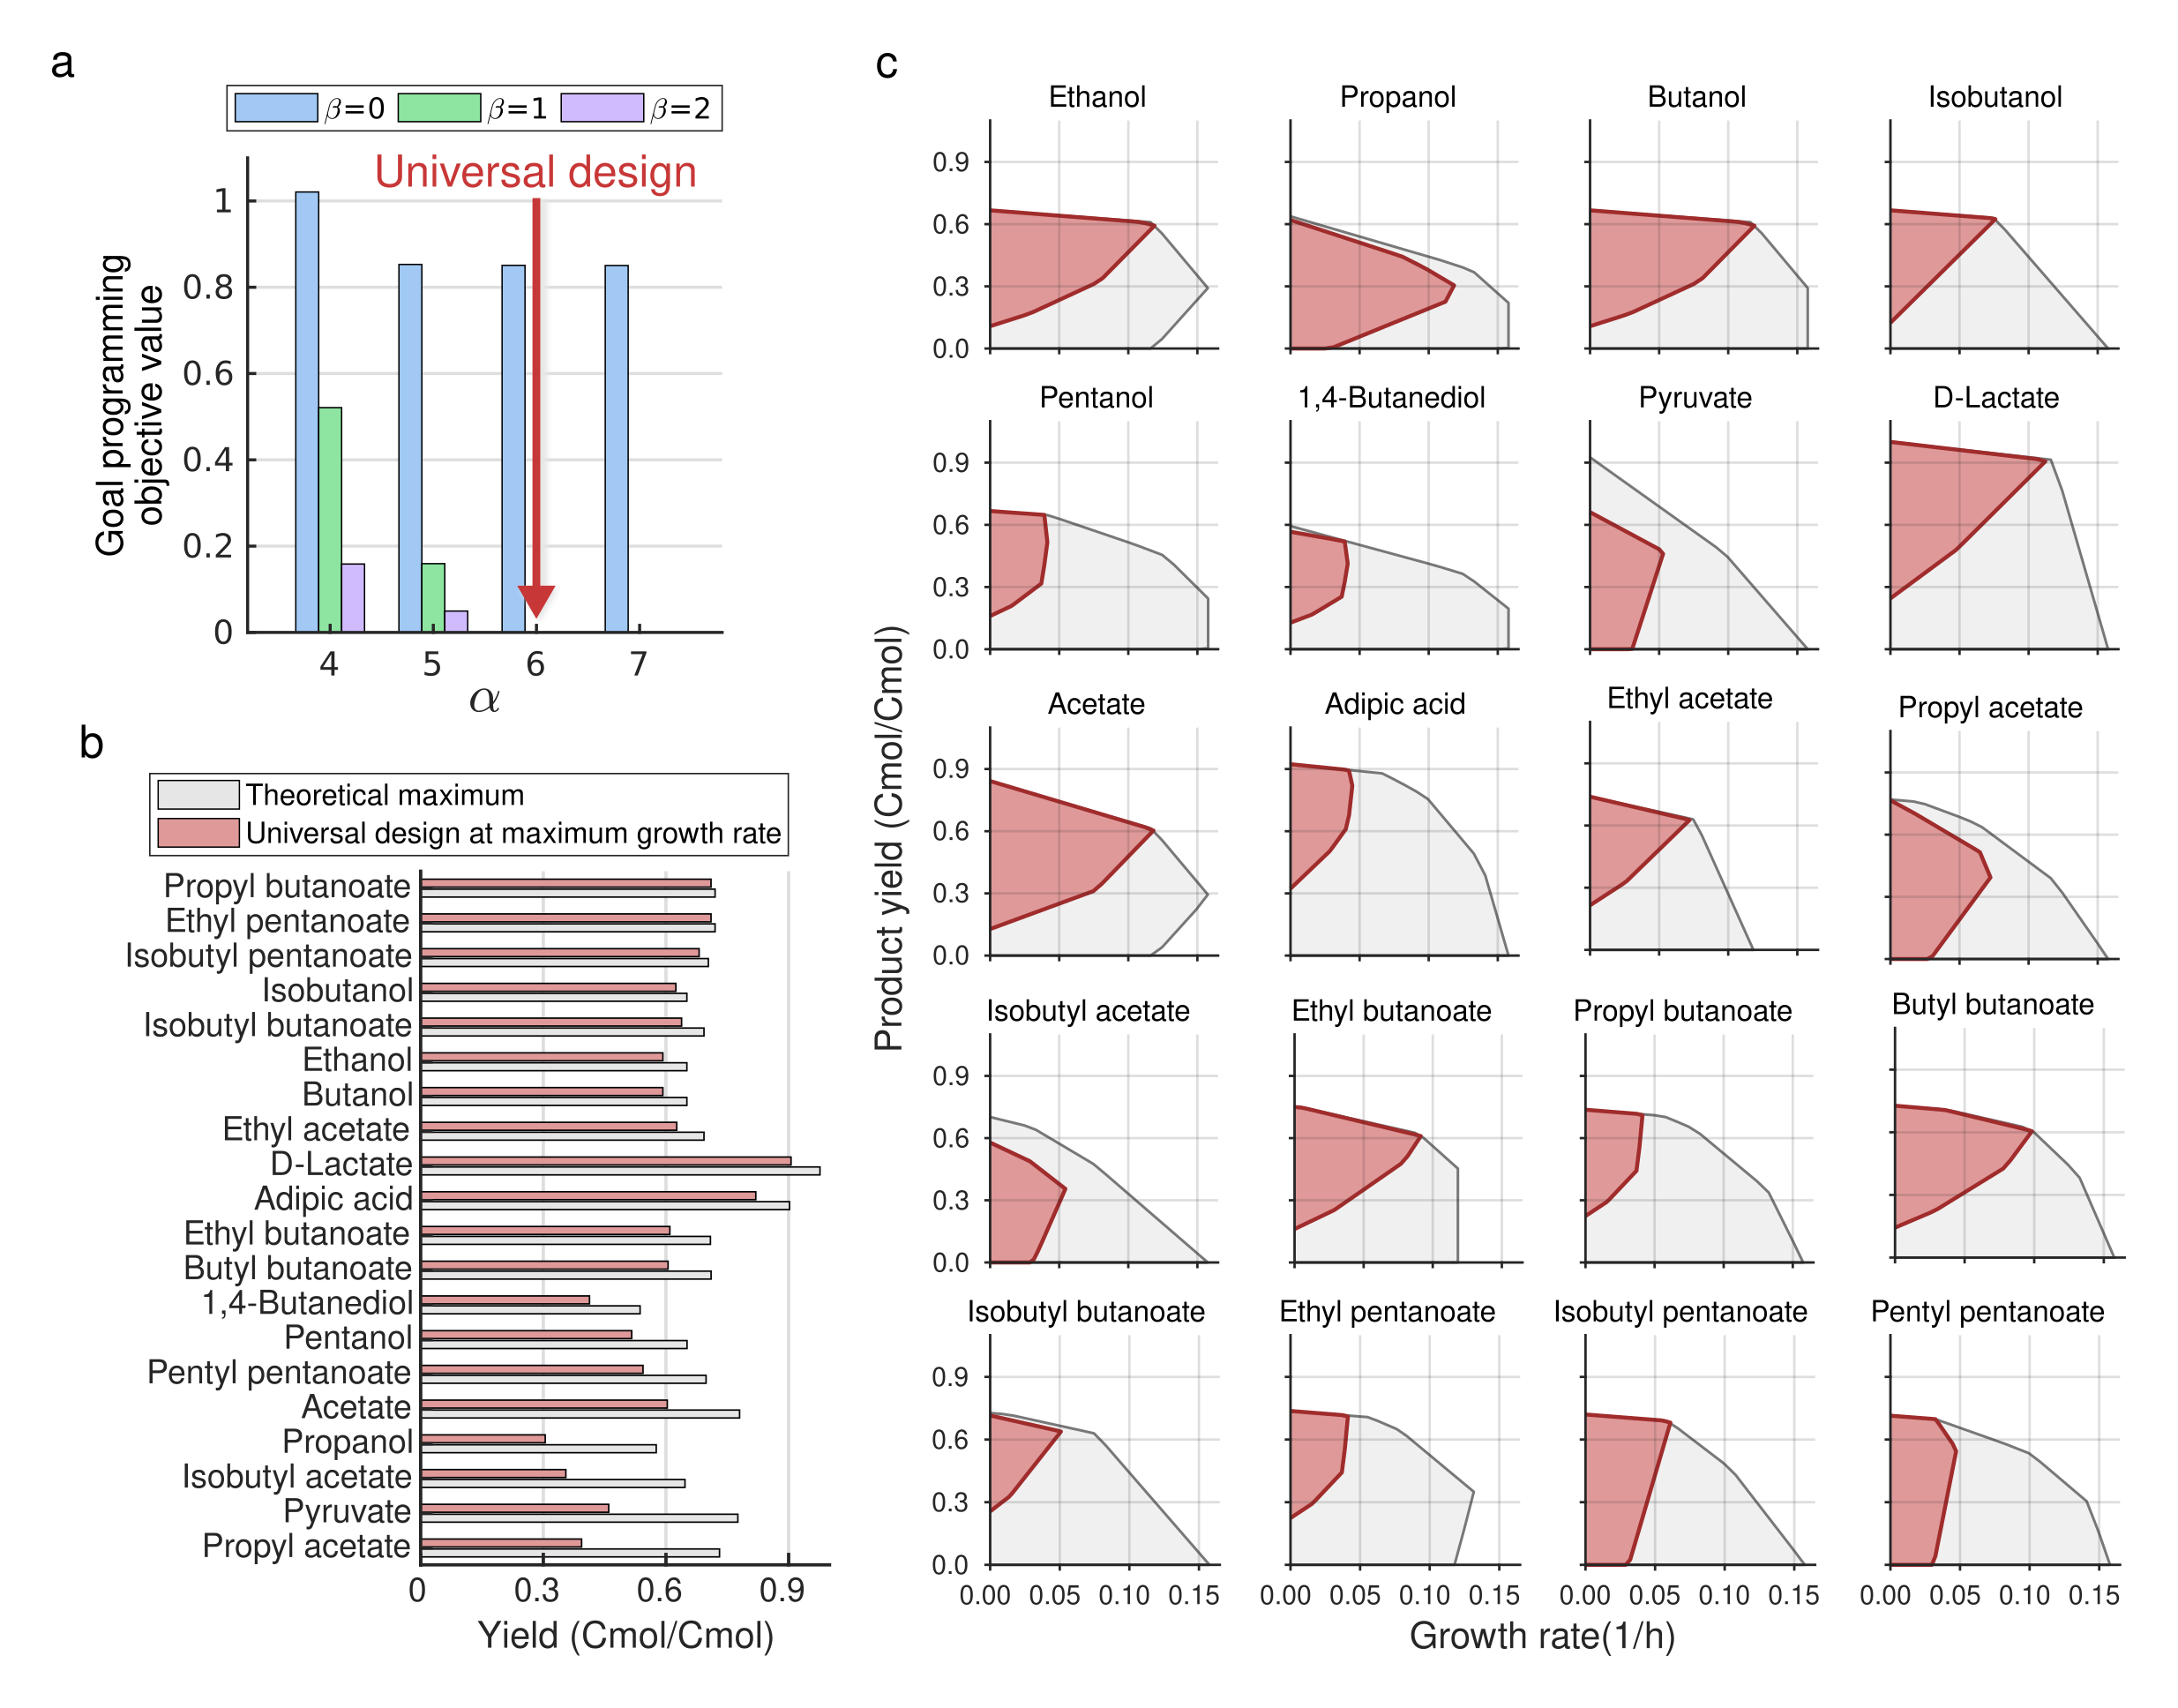
\includegraphics[width=\textwidth,keepaspectratio]{universal-design.png}
    \caption[Identification of a universal modular cell compatible with all production modules under the \textit{wGCP} design phenotype]{Identification of a universal modular cell compatible with all production modules under the \textit{wGCP} design phenotype. (a) Goal programming solutions with increasing $\alpha$ and $\beta$ values. The goal programming objective value \eqref{eq5:goal_obj} in the y-axis measures the difference between the performance of production strains and the target goal, i.e., $\sum_{k\in \{ k \in \mathcal{K}: f'_k < g_k\}}(f'_k - g_k)$ where the target goal is set to be $g_k=0.5$. The parameters $\alpha=6$ and $\beta=1$ are sufficient to identify a universal modular cell design meeting the required goal for all production networks. (b) Comparison between the yield performances of the designed modular production strains and maximum theoretical values. (c) The feasible flux spaces for the wild-type (gray) and designed modular production strains (crimson). Based on the \textit{wGCP} design phenotype, to increase growth rate, each mutant must increase product synthesis rate. The genetic manipulations of this universal modular cell design are indicated in the metabolic map of Figure~\ref{fig5:core-modules}c.}
    \label{fig5:universal-design}
%\end{adjustwidth}
\end{figure}
%}

\subsection{Flexible metabolic flux capacity of \textit{E. coli} core metabolism enables the design of a universal modular cell}

\subsubsection{Interface reactions responsible for metabolic flexibility of a universal modular cell are identified by comparing flux distributions of production networks}
The designed universal modular cell (Figure~\ref{fig5:universal-design}) can theoretically adapt to the conflicting metabolic requirements of all production modules (Table~\ref{tab5:pathways}).
To gain further insight into this unique metabolic capability of the modular cell, we analyzed the simulated \emph{reference flux distributions} of each production network using the \emph{flux variance clustering} (FVC) analysis (Materials and Methods).
Reactions with the highest flux changes across the production networks are likely critical for the proper operation of the universal modular cell and might present potential bottlenecks.
Such reactions were identified by filtering their reference flux standard deviation calculated across production networks with an \textit{ad hoc} threshold of 0.2 (mol/substrate mol).
Over 90\% of the 535 active reactions, each of which carries a non-zero flux in at least one production network, had standard deviation values below the threshold, indicating  highly conserved metabolic core pathways among production networks. Only 9.5\% of the active reactions presented a standard deviation magnitude above the threshold (Figure~\ref{fig5:core-modules}a).


\begin{table}[ht]
%\begin{table}[!ht]
%\begin{adjustwidth}{-2.25in}{0in}
    \caption[Overall production module pathway stoichiometries and associated simulated secretion fluxes of the universal modular cell design]{Overall production module pathway stoichiometries and associated simulated secretion fluxes of the universal modular cell design.
    DoR is the degree of reduction of the final product (mol~$e^-$ / mol~C). Metabolite secretion profiles are determined from the simulated reference flux distributions (mol~C / mol~C) of the universal modular cell design.
    Flux abbreviations: $r_{p}$, product; $r_{ac}$, acetate; $r_{co_2}$, CO$_2$; $r_{for}$, formate; $r_{succ}$, succinate.
    Note that the negative CO$_2$ fluxes in pyruvate and acetate production networks indicate overall CO$_2$ uptake enabled by phosphoenolpyruvate carboxylase (PPC).}
    \centering
 	%Table : Production networks overall reactions and secreted product yields for the reference flux distributions of the universal design.

\rowcolors{2}{gray!25}{white}
\resizebox{\textwidth}{!}{\begin{tabular}{lcccccc}
\toprule
    Overall reaction  & DoR  & $r_{p}$ & $r_{ac}$ & $r_{co_2}$ & $r_{for}$ & $r_{succ}$ \\
\midrule
pyr + nadh $\rightarrow$ \textbf{ethanol} $|$  accoa + 2 nadh $\rightarrow$  \textbf{ethanol} (native) 		&7.0&0.58&0.01&0.27&0.04&- \\
oaa + glu  + 2 atp + 2 nadph  +  nadh $\rightarrow$ akg + \textbf{propanol}					&6.7&0.31&0.36&0.07&0.18&- \\
2 accoa + 4 nadh $\rightarrow$ \textbf{butanol}									&6.5&0.59&0.01&0.28&0.04&- \\
2 pyr + nadph + nadh $\rightarrow$  \textbf{isobutanol}								&6.5&0.62&-&0.31&-&- \\
oaa + glu  + accoa + 3 nadh + 2 atp + 2 nadph $\rightarrow$ akg + \textbf{pentanol}				&6.4&0.50&0.21&0.24&0.03&- \\
succ  + akg + atp + 4 nadh + accoa  $\rightarrow$  ac + \textbf{1,4-butanediol}					&5.5&0.46&0.33&0.17&-&- \\
$\rightarrow$ \textbf{pyruvate}											&3.0&0.46&-&-0.16&-&0.66 \\
pyr + nadh $\rightarrow$ \textbf{D-lactate}									&3.7&0.91&-&-&-&- \\
accoa  $\rightarrow$  atp + \textbf{acetate}									&3.5&0.60&0.60&-0.30&0.61&- \\
accoa + succoa + 2 nadh $\rightarrow$  atp + \textbf{adipic acid}						&4.0&0.82&0.05&0.04&0.06&- \\
accoa + pyr + nadh $\rightarrow$ \textbf{ethyl acetate}								&5.0&0.63&-&-&0.32&- \\
accoa + oaa + glu  + 2 atp + 2 nadph  +  nadh $\rightarrow$ akg + \textbf{propyl acetate}			&5.2&0.41&0.30&-&0.24&- \\
accoa + 2 pyr + nadph + nadh $\rightarrow$ \textbf{isobutyl acetate}						&5.3&0.36&-&0.02&0.06&0.52 \\
2 accoa + 3 nadh  + pyr $\rightarrow$ \textbf{ethyl butanoate}							&5.3&0.61&-&0.09&0.23&- \\
2 accoa + 3 nadh  + oaa + glu  + 2 atp + 2 nadph  $\rightarrow$ akg + \textbf{propyl butanoate}			&5.4&0.68&0.03&0.23&0.04&- \\
4 accoa + 6 nadh  $\rightarrow$ \textbf{butyl butanoate}							&5.5&0.61&-&0.14&0.18&- \\
2 accoa + 3 nadh  + 2 pyr + nadph $\rightarrow$ \textbf{isobutyl butanoate}					&5.5&0.64&-&0.16&0.16&- \\
oaa + glu  + accoa +  2 nadh + 2 atp + 2 nadph  + pyr $\rightarrow$  akg + \textbf{ethyl pentanoate}		&5.4&0.68&0.03&0.23&0.04&- \\
oaa + glu  + accoa + 2 nadh + 2 atp + 3 nadph + 2 pyr $\rightarrow$ akg + \textbf{isobutyl pentanoate}		&5.6&0.67&0.01&0.25&0.03&- \\
2 oaa + 2 glu  + 2 accoa +  4 nadh + 4 atp + 4 nadph  $\rightarrow$ 2 akg + \textbf{pentyl pentanoate}		&5.6&0.53&0.22&0.20&0.02&- \\
\hline
\end{tabular}}

    \label{tab5:pathways}
%\end{adjustwidth}
\end{table}

In our case study of designing a universal modular cell compatible with all 20 production modules, unbiased hierarchical clustering (Figure~\ref{fig5:core-modules}b) revealed the presence of four interface reaction types in the core metabolism of \textit{E. coli} that are activated to fit specific production modules (Figure~\ref{fig5:core-modules}c).
In the context of chassis metabolism, an endogenous module corresponds to a reaction or group of highly coupled reactions that become active to accomplish a certain metabolic function.
The interface reaction classification can be understood in terms of location (i.e., proximity in the metabolic network) and three metabolic functions. The first function is the direction of carbon towards general precursor metabolites including (i) pyruvate and acetyl-CoA captured by acetyl-CoA-associated modules and (ii) oxaloacetate, succinate, succinyl-CoA, and $\alpha$-ketoglutarate captured by TCA-associated modules. The second function is the direction of carbon from the precursor metabolites towards secretable molecules, captured by the upstream and TCA-associated modules. The third function is the use of ATP- and NADP(H)-dependent pathways required to maintain homeostasis, captured by the acetyl-CoA-associated and energetic modules. While these functions are conceptually separable, their biochemical manifestation overlaps, i.e., specific metabolic reactions or pathways can simultaneously fulfill several functions.

Interface reactions enable the exchangable production modules to properly operate with the universal modular cell.
These interface reactions might become potential metabolic bottlenecks in practice if they cannot satisfy the predicted fluxes, and thus might be critical engineering targets when the associated production modules are used.


\paragraph{Acetyl-CoA-associated interface reactions.}
This interface type contains pyruvate formate lyase (PFL) and pyruvate dehydrogenase enzyme complex (PDH) reactions that convert pyruvate to acetyl-CoA.
Intuitively, products derived from pyruvate, such as isobutanol, require a low flux through PFL and PDH while those derived from acetyl-CoA require a high flux.
Remarkably, the redox states of production strains determine the ratios of PFL to PDH  fluxes.
For example, the ethanol production network has a relatively high flux through PDH and a low flux through PFL; however, for ethyl acetate that has a lower degree of reduction than ethanol (Table~\ref{tab5:pathways}), PFL with formate secretion is prioritized over PDH with NADH  generation.
Note that our model did not include the regulatory restriction that PDH is inhibited in \textit{E. coli} anaerobically because the function of PDH is equivalent with the coupling of PFL and heterologous NADH-dependent formate dehydrogenase (FDH) demonstrated experimentally for increased butanol\citep{shen2011, nielsen2009} and pentanol\citep{tseng2012} production.

\paragraph{Upstream interface reactions.}
This module  type is formed by reactions located directly upstream of a secretable metabolite, often associated with the target production module, and thus provides the necessary precursor metabolite(s). Such reactions are commonly over-expressed in practice, e.g., the ECOAH1-HACD1-ACACT1r interface reaction group (comprising of 3-hydroxyacyl-CoA dehydratase, 3-hydroxyacyl-CoA dehydrogenase, and acetyl-CoA acetyl transferase) responsible for generating butyryl-CoA and  the ACLS-DHAD1-KARA1 interface reaction group (comprising of acetolactate synthase, dihydroxy-acid dehydratase, and keto-acid reductoisomease) responsible for generating isobutyryl-CoA.
These interface reactions can also become active to form byproducts in certain production networks, e.g., the PTAr-ACKr-ACT2rpp-ACtex interface reaction group (comprising of phosphate acetyl transferase, acetate kinase, and cytosolic and periplasmic acetate transport) that not only carries the highest flux in the acetate production network but also becomes active in the propanol-associated modules.

\paragraph{TCA-associated interface reactions}
This interface type has the same function as the upstream interface reactions but it is localized in the TCA (Krebs) cycle.
Several products, including adipic acid, 1,4-butanediol, propanol, pentanol, and their associated esters, are derived from the TCA intermediates and interface with the universal modular cell via the TCA-derived interface reactions.
The SUCOAS-MMM-MMCD interface reaction group (comprising of succinyl-CoA synthetase, Methylmalonyl-CoA mutase, methylmalonyl-CoA decarboxylase) must be activated to convert succinate into succinyl-CoA and then propanoyl-CoA. Remarkably, two routes are present to synthesize fumarate from oxaloacetate, including the conventional MDH-FUM interface reaction group (comprising of malate dehydrogenase and fumarase) that consumes NADH and the cyclic ASPTA-GLUDY-ASPT interface reaction group (comprising of aspartate transaminase, glutamate dehydrogenase, and L-aspartase) that consumes NADPH. These NADH/NADPH cofactors are not interchangeable due to the deletion of the transhydrogenase THD2pp in the universal modular cell, so the isobutyl pentanoate and pentyl pentanoate modules, that are derived from the ASPTA-GLUDY-ASPT interface reaction group, also have a high NADPH requirement. Some production networks, such as pyruvate and isobutyl acetate that are not based on the TCA-derived interface reactions, secrete succinate instead of ethanol and/or lactate to balance redox by using the PPC-MDH-FUM-SUCCtex interface reactions (comprising of phosphoenolpyruvate carboxylase, malate dehydrogenase, fumarase, and succinate transport).

\paragraph{Energetic interface reactions}
This interface type primarily involves NAD(P)-dependent transhydrogenase (THD2pp) and ATP synthase (ATPS4rpp). Other reactions that allow coupling of phosphate- and electron-transfer cofactors are also included. The reactions in this module help buffer the diverse electron and ATP requirements of production networks. THD2pp is deleted in the chassis but used as a module reaction in the isobutanol and acetate production networks.
In the case of isobutanol production, transhydrogenase expression has been demonstrated to increase the synthesis of NADPH and thus isobutanol \citep{shi2013}.
Acetate has the smallest degree of reduction after pyruvate, which results in redox imbalance that is compensated via formate secretion. In conjunction with these mechanisms, ATPsynthase works in the reverse direction by hydrolyzing excess ATP. Other production networks also use ATPS4rpp to eliminate excess ATP as observed, for example, in the ethyl acetate production network. This strategy is consistent with ATP wasting approaches recently demonstrated \citep{hadicke2015}.

%\afterpage{%
%\begin{figure}[H]
%    \caption{\textit{Caption on next page.}}
%	\centering
%    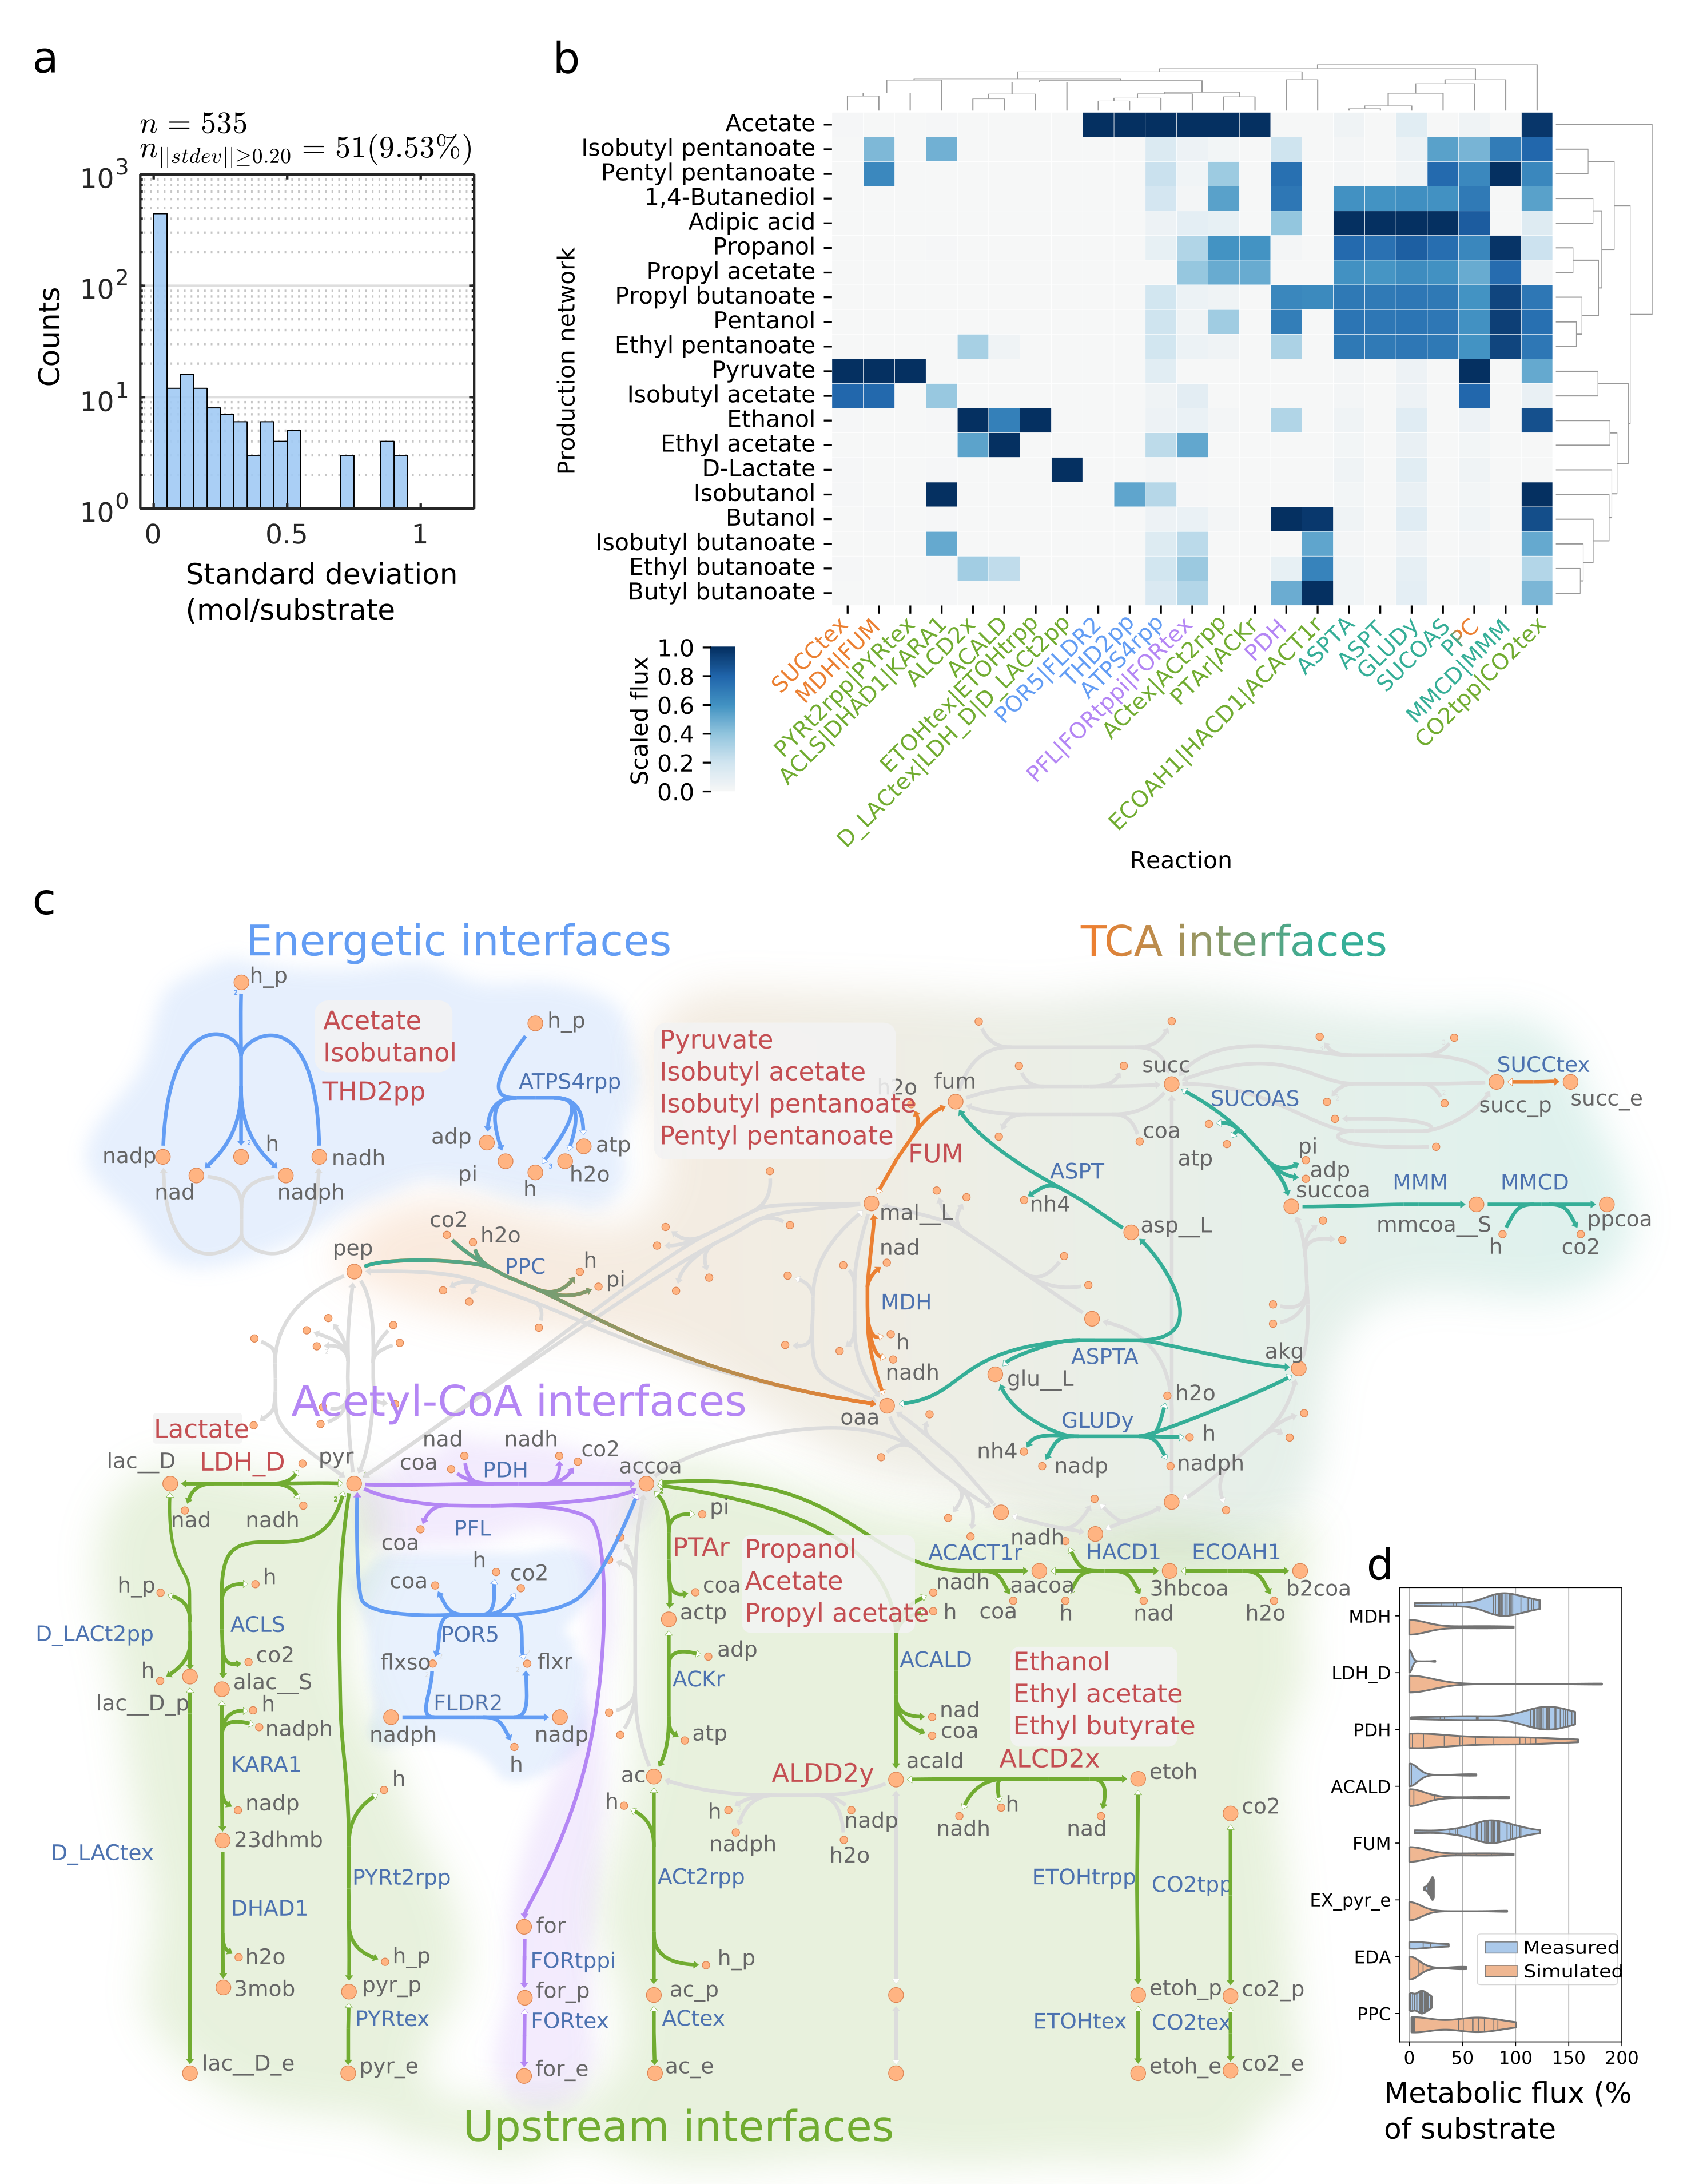
\includegraphics[height=\textheight,keepaspectratio]{core-modules.png}
%\end{figure}
%
%\addtocounter{figure}{-1}
\begin{figure}[!hp]
    \centering
    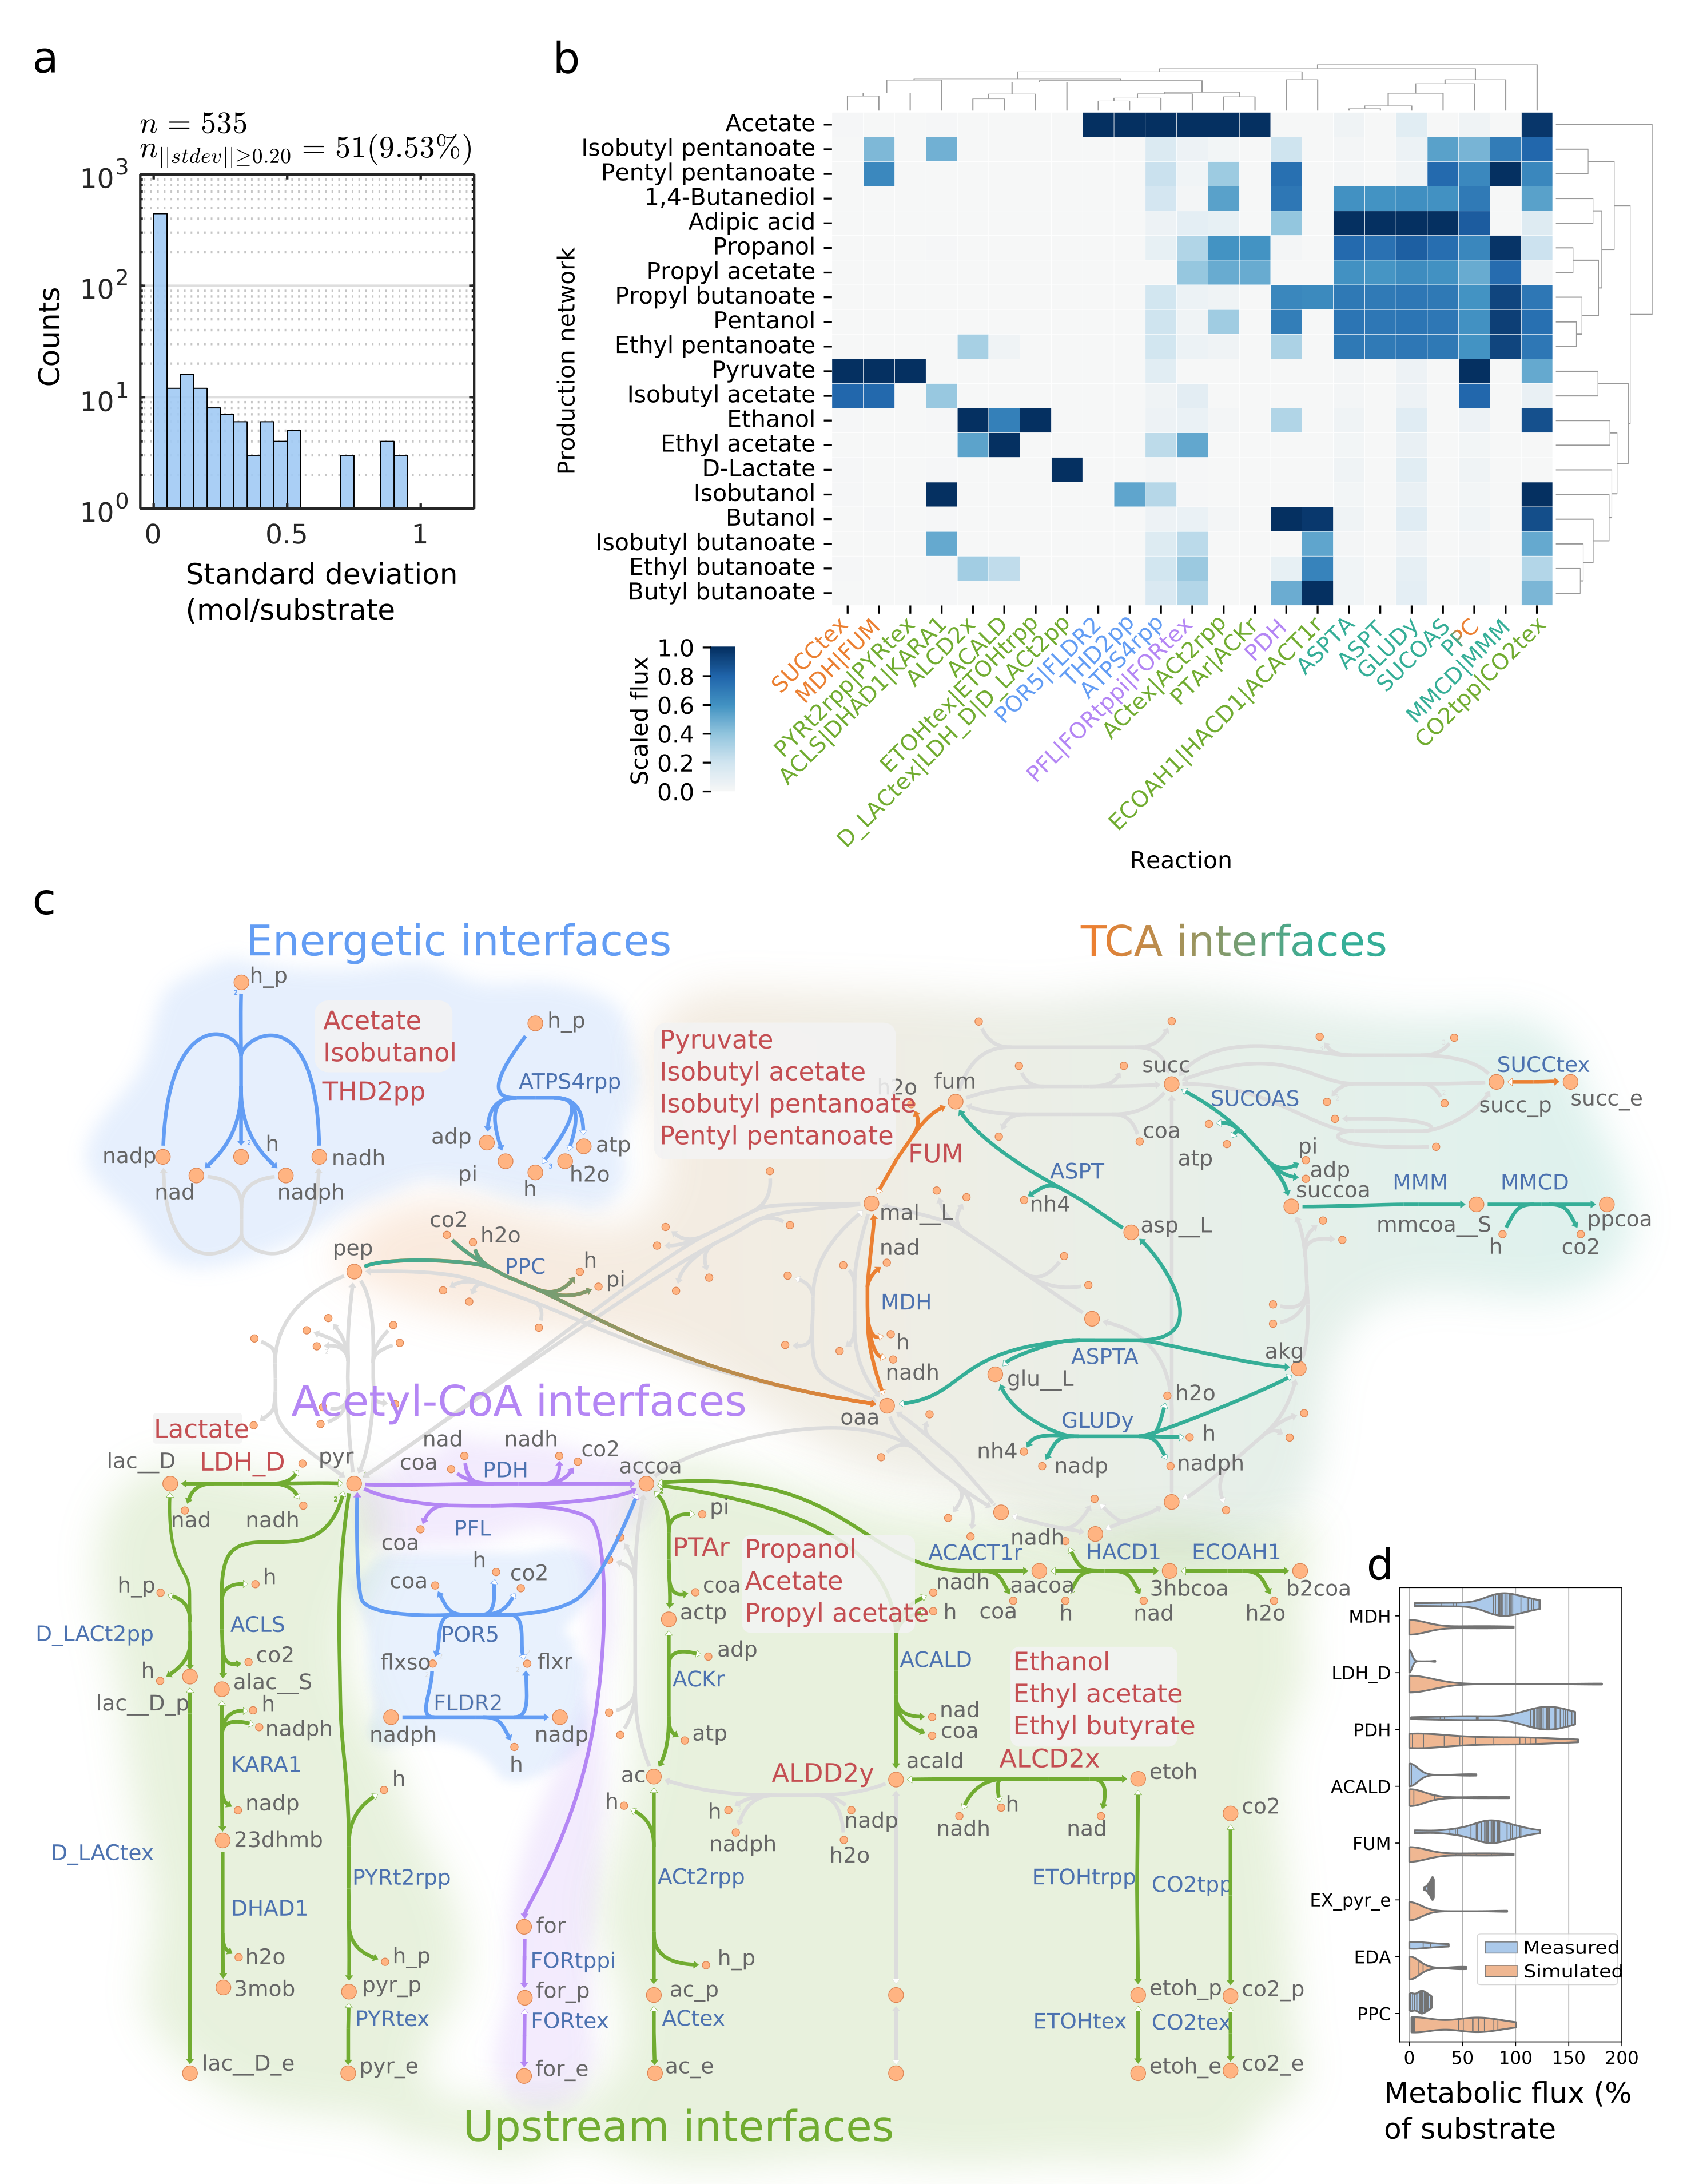
\includegraphics[height=.77\textheight,keepaspectratio]{core-modules.png}
    \caption[Flexible metabolic flux capacity of \textit{E. coli} metabolism enables the universal modular cell design]{\textbf{Flexible metabolic flux capacity of \textit{E. coli} metabolism enables the universal modular cell design.} (a) Standard deviation of each reaction flux  across production networks. (b) Scaled fluxes of the 51 reactions with standard deviation magnitude above 0.2,  excluding proton, water transport, and exchange reactions. A scaled flux for a reaction is determined by the reference flux distribution value divided by the maximum value of that reaction across all production networks. Hence, a scaled flux of 0 indicates a given reaction does not carry any flux, and a scaled flux of 1 indicates that this reaction carries the highest flux across production networks.  (c) Interface reactions of the universal modular cell.  The reactions colored in red are deleted in the chassis, but are used as module reactions in the production networks shown in the adjacent gray boxes.  (d) Comparison between simulated and measured fluxes. The solid lines within the ``violins" correspond to samples.
    }
    \label{fig5:core-modules}
\end{figure}
%}

\subsubsection{Comparison between simulated and measured intracellular fluxes reveals flexible metabolic flux capacity of \textit{E. coli} to accommodate the required wide flux ranges} \label{sec:flux_comparison}

Flux analysis of the production networks suggests that the core metabolic reactions (Figure~\ref{fig5:core-modules}b) require a wide range of fluxes when coupled with different production modules. To successfully implement this modular design in practice, we need to evaluate whether the metabolism of \textit{E. coli} has the inherent metabolic flux capacity to accommodate these required fluxes.
We compared the simulated reference flux distributions with a recent collection of 45 measured metabolic fluxes \citep{khodayari2016} that are collected from multiple studies across various conditions (e.g., growth under aerobic and anaerobic conditions, use of glucose or acetate or pyruvate as a carbon source) and genotypes (e.g., wild-type \textit{E. coli} and mutants with single gene deletions) \citep{ishii2007, kabir2005, zhao2004, zhao2003}.
Note that while the experimental data set provides a flux distribution baseline for wild-type and relatively small deviations for single gene deletion mutants, we anticipate that highly engineered strains with more gene deletions are likely to exhibit wider flux distributions.

Within the reactions present in the 23 groups that constitute interface reactions (Figure~\ref{fig5:core-modules}b), 8 reactions also appeared in the experimental dataset (Figure~\ref{fig5:core-modules}d).
Remarkably, a highly consistent overlap of flux ranges was observed between the simulated and measured fluxes for malate dehydrogenase (MDH), pyruvate dehydrogenase (PDH), acetaldehyde dehydrogenase (ACALD), fumarase (FUM), and 2-dehydro-3-deoxy-phosphogluconate aldolase (EDA).
For the cases of  D-lactate dehydrogenase (LDH\_D), and pyruvate secretion (EX\_pyr\_e) that are directly coupled with the biosynthesis of lactate and pyruvate, respectively, we observed the maximum simulated fluxes surpass the measured values, suggesting that further engineering of wild-type and single-gene deletion \textit{E. coli} is needed to attain the requried fluxes.
Indeed, previous studies\citep{zhou2003, causey2004} have been able to redirect metabolic fluxes in \textit{E. coli} for yields of lactate and pyruvate above 75\% of the theoretical maximum values by simultaneous elimination of competing fermentative pathways for biosynthesis of acetate ($\Delta$\textit{ackA}), formate ($\Delta$\textit{pflB}), and ethanol ($\Delta$\textit{adhE}).
The only remaining discrepancy between the simulated and measured fluxes is PPC.
Studies, not included in the comparison data set, have reported up to 50\% more PPC flux observed under aerobic conditions \citep{peng2004, siddiquee2004}, which is still considerably below several of the simulated fluxes.
This result suggests that PPC can be a potential metabolic bottleneck in certain production modules. One possible solution is to include in the affected production modules the heterologous PPC from \textit{Actinobacillus succinogenes} which has been successfully over-expressed in \textit{E. coli} for increased succinate production \citep{kim2004}.
Additionally, bacterial PPC activity can be increased by elevating the acetyl-CoA pool \citep{lin2004}.


% Note: Most of the fluxes are aerobic, which may explain some of the bias in particular with LDH_D, however this can also be a source of challenge, since the design is anaerobic. Also the fluxes of engineered strains with most fermentative products remove can be very different, and such strains are not necessarily included here, but the type of strain we are analyzing has 6 knockouts. Also some fluxes in W.T. seem to be widely different among studies.

\subsubsection*{Random sampling of metabolic fluxes confirms the narrow operation range of interface reactions}
The reference flux distributions analyzed so far represent the ideal metabolic states for each production strain. However, other metabolic states might also exist.
To address this uncertainty, we performed randomized flux sampling \citep{kaufman1998, heirendt2017} for each production network under the constraint that product synthesis rate must be above 50\% of the maximum value.
The results show that the metabolic flux distributions (S.M. 1 - Figure S2) for most reactions involved in the interface reactions are very narrow, except for the two alternative pathways of ethanol biosynthesis, i.e., the endogenous PDH-ACALD-ALCD2x route comprising of pyruvate dehydrogenase, acetaldehyde dehydrogenase, and alcohol dehydrogenase (Figure~\ref{fig5:sampling}a) and the heterologous PYRDC-ALCD2x route comprising of pyruvate decarboxylase and alcohol dehydrogenase. These two pathways can be used interchangeably in the ethanol production network, where there is a linear correlation between PYRDC and PDH fluxes (Figure~\ref{fig5:sampling}b). Notably, the sampled fluxes cannot indicate preferential use of either the ethanol synthesis route because the model does not take into account of kinetic ($k_{\textrm{cat}}$, $k_\textrm{M}$) and regulatory constraints.
%Furthermore, the sampled fluxes do not capture the extremes where only of the two alternative pathways is used, this could be indicative of a possible biological phenomenon or introduced by a bias in flux sampling towards high volume regions of the solution space.
In summary, even though interface reactions must have flexible metabolic flux capacities to enable a universal modular cell to be compatible with various exchangeable production modules, they must also operate within in a narrow flux range when interfacing with a specific production module.

%\afterpage{%
%\paragraph{Figure S2}
\begin{figure}[!hp]
    \centering
    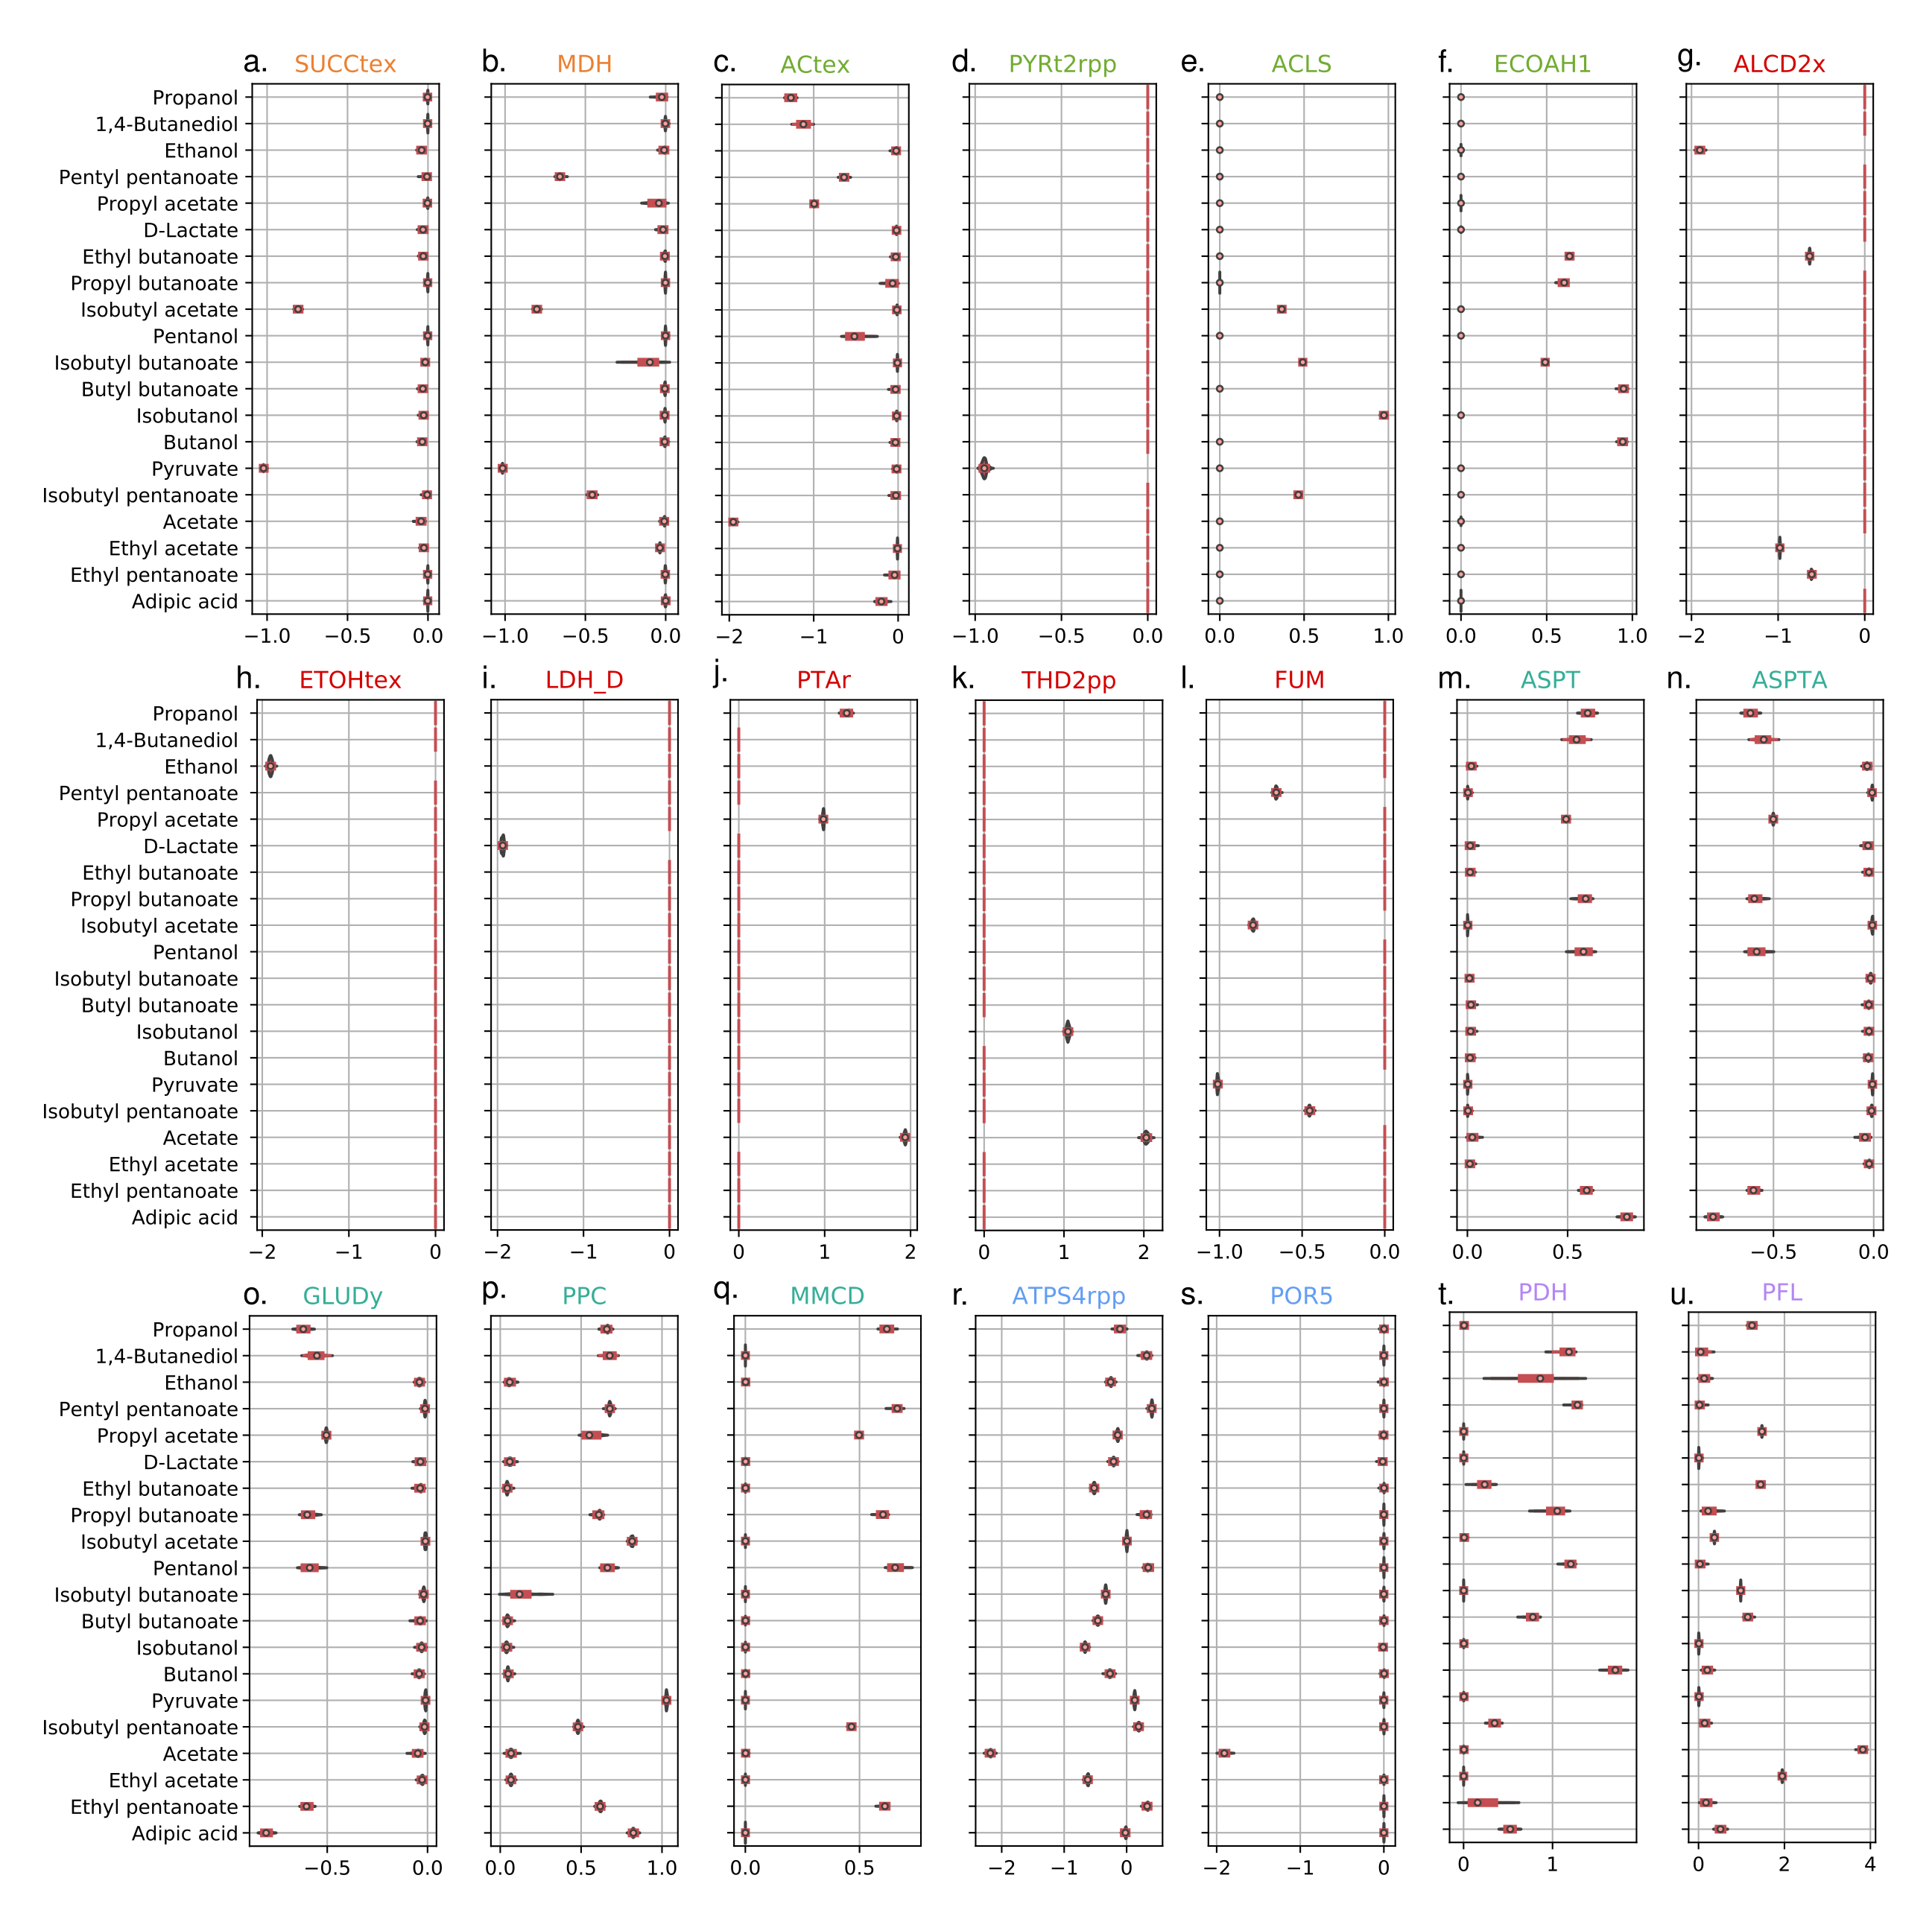
\includegraphics[width=\textwidth,height=\textheight,keepaspectratio]{Figure-S2}
    \caption[Violin plot of sampled reaction flux distributions]{
Violin plot of sampled reaction flux distributions. Reaction colors are consistent with Figure~\ref{fig5:core-modules}. The flux of SUCOAS could not be sampled since this reaction is involved in a thermodynamically infeasible cycle.
    }
    \label{fig5:fig-s2}
\end{figure}
%}

%\afterpage{%
\begin{figure}[!ht]
    \centering
    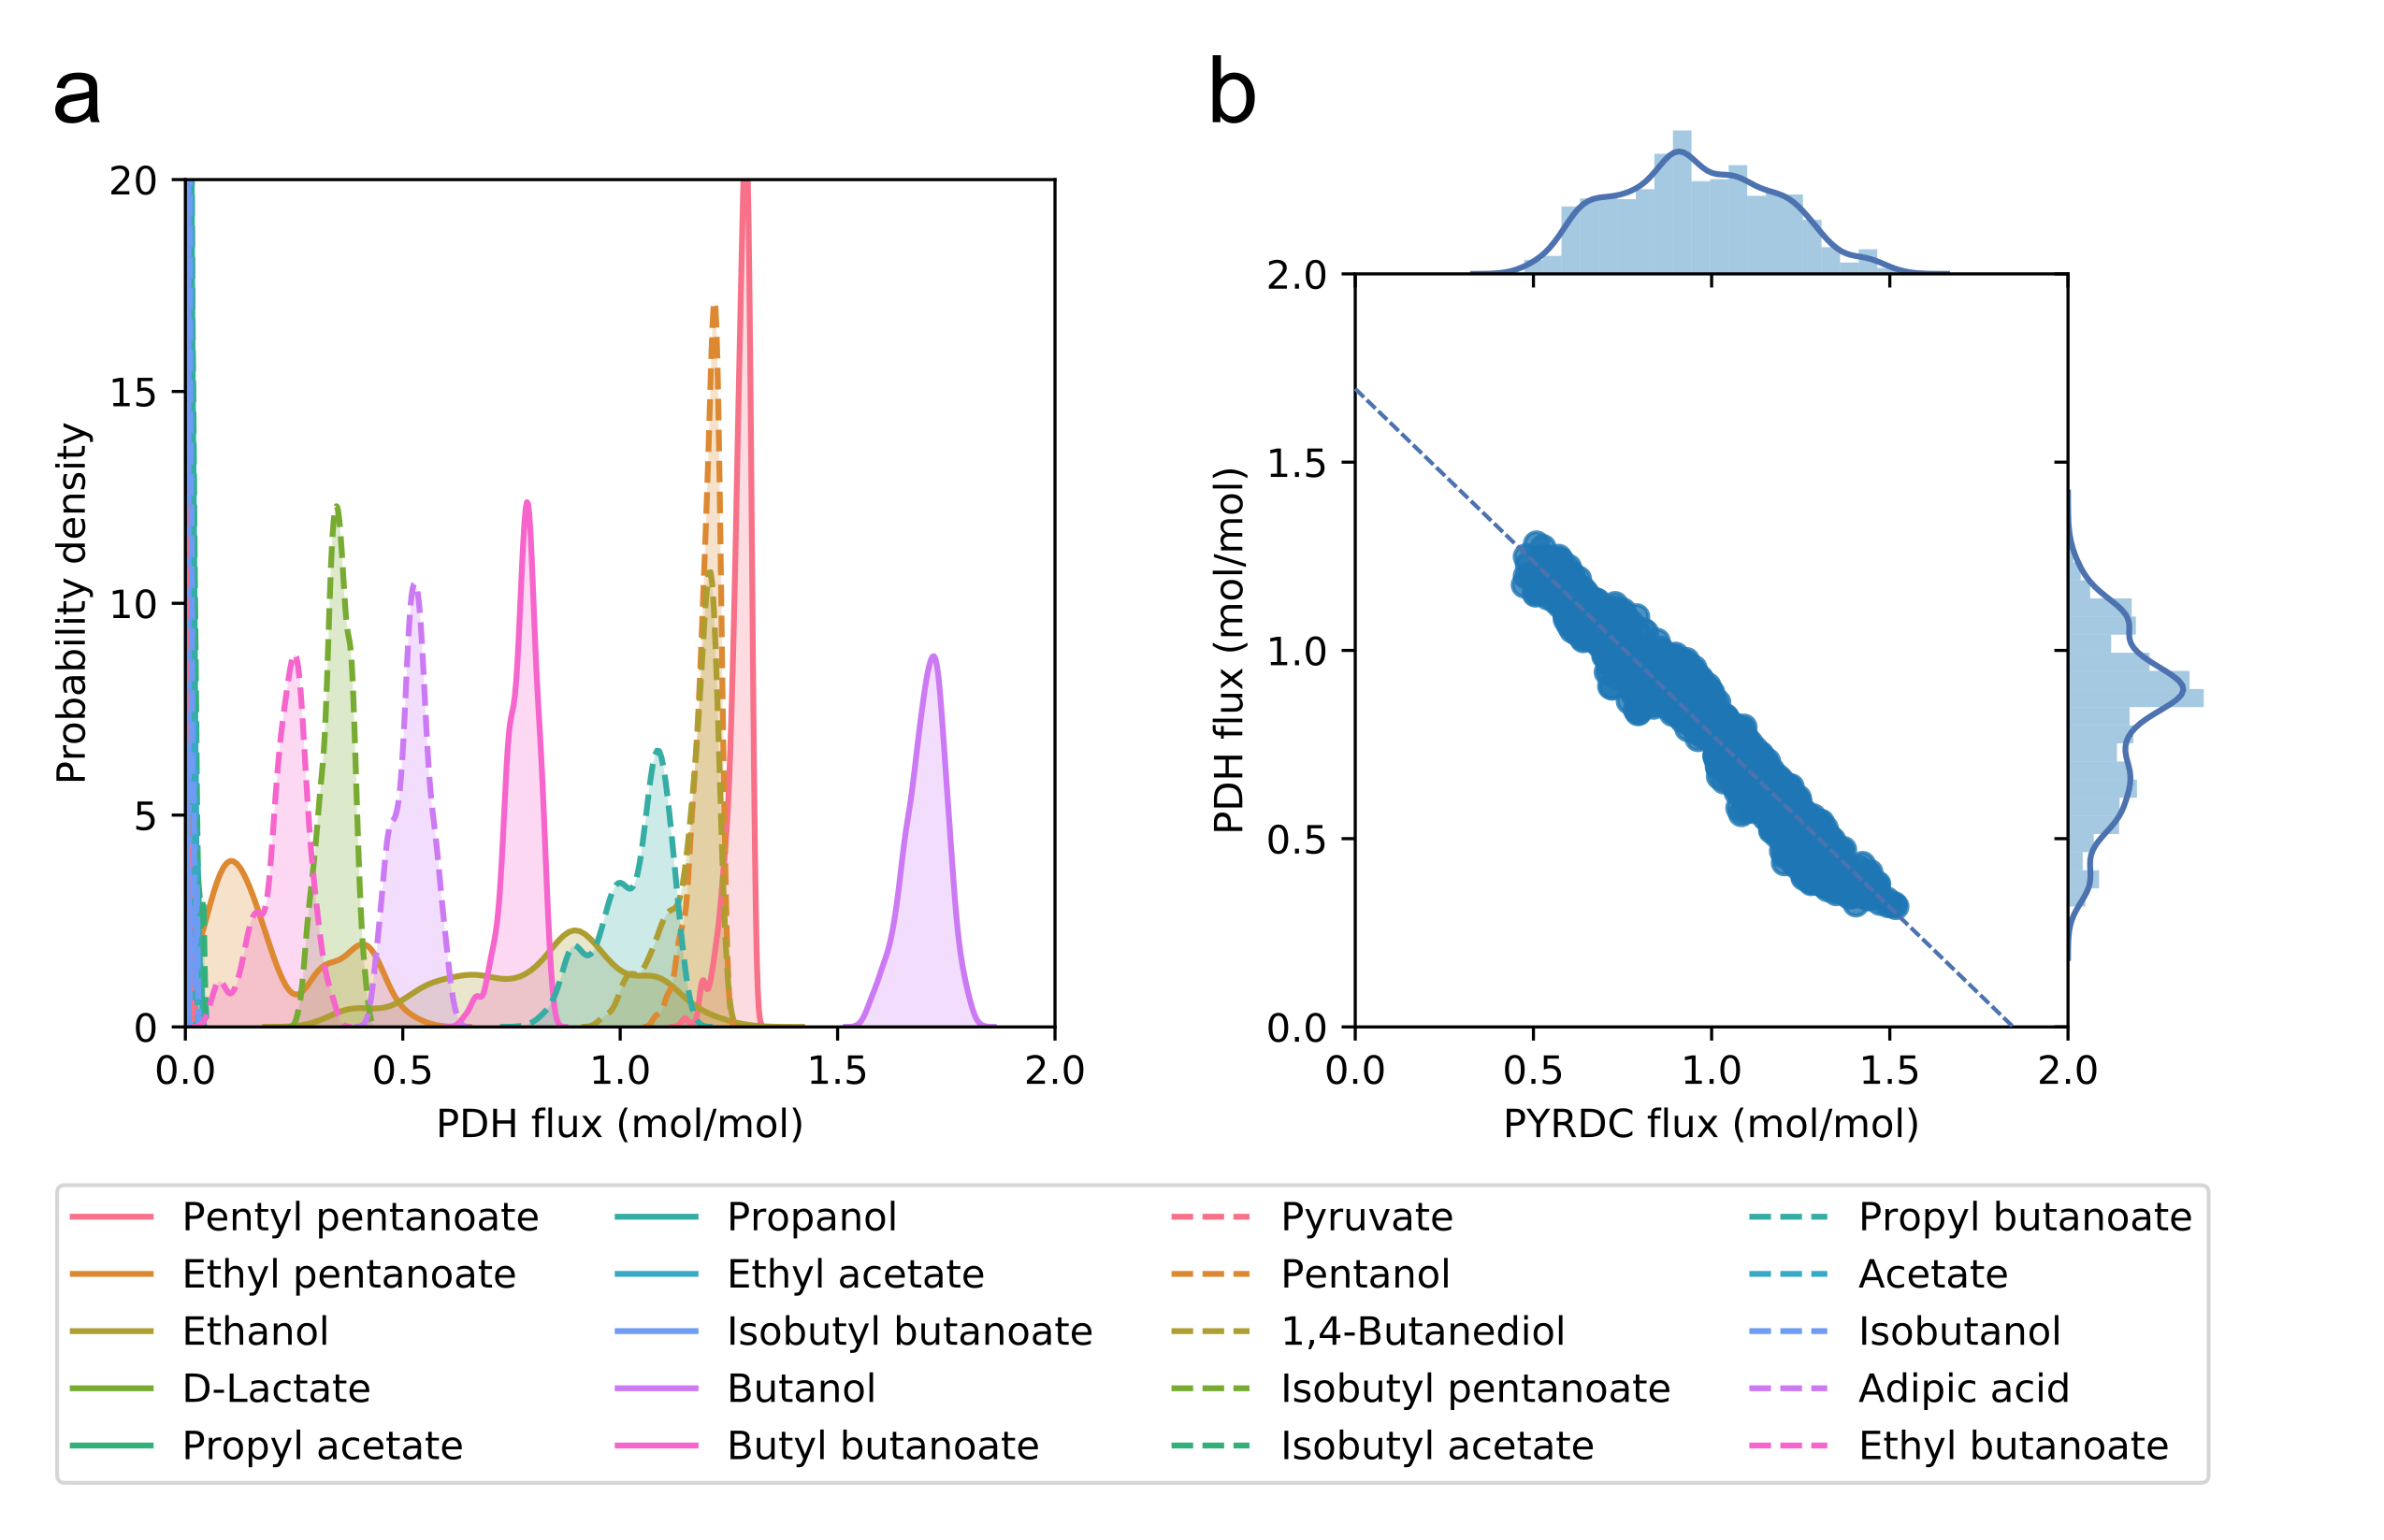
\includegraphics[width=.9\textwidth,keepaspectratio]{ethanol_sampling.png}
    \caption[Sampled flux distributions of the ethanol biosynthesis pathways]{Sampled flux distributions of the ethanol biosynthesis pathways. (a)~Probability density function of sampled fluxes for pyruvate dehydrogenase (PDH) across all production networks. Note that ethanol and ethyl pentanoate have the widest operation range. (b)~Sampled metabolic fluxes of pyruvate decarboxylase (PYRDC) and PDH in the ethanol production network.}
    \label{fig5:sampling}
\end{figure}%}


\section{Conclusions}
In this study, we formulated multi-objective modular strain design as blended and goal attainment optimization problems. These problems can be solved by MILP algorithms that guarantee Pareto optimal solutions, exhaustively search the space of alternative solutions, and specify design requirements such as module prioritization or universal compatibility.
This multi-objective strain design approach can be extended with additional design variables (e.g., up- and down-regulation\citep{pharkya2004} or reaction insertion from database\citep{pharkya2006}) or alternative flux prediction models\citep{chowdhury2014,dinh2018} to expand its applications, including use of exchangeable metabolic modules for bioremediation  and biosensing.
In terms of biological significance, the ModCell2-MILP and FVC methods developed could identify a universal modular cell that harnesses the inherent modularity and flexibility of native \textit{E. coli} metabolism to properly interface with a variety of biochemically diverse pathways. This universal design was predicted to display a growth-coupled-to- product-formation phenotype for all pathways, enabling its use as a platform for pathway optimization through high-throughput library selection and/or adaptation. The feasibility of this universal design strategy is found to be consistent with experimental evidence of isolated metabolic engineering strategies towards target products and measured intracellular flux ranges. Furthermore, analysis of the metabolic fluxes in this universal design revealed clusters of reactions in central metabolism, named interface reactions, that become activated to interact with specific pathways, providing a mechanistic view into the modularity of metabolic pathways.
In this study, the universal design developed was limited to a library of 20 molecules in \textit{E. coli} because one primary aim was to compare the MILP solution with the MOEA solution previously presented. Future studies will use the developed methods to design and understand modularity for different organisms and a larger library of product synthesis modules.



% Include only the SI item label in the paragraph heading. Use the \nameref{label} command to cite SI items in the text.
\section*{Supporting information}

\paragraph{File S1}
\textbf{Spreadsheet with modular cell designs for \textit{E. coli} core model.}

\paragraph{File S2}
\textbf{Computer programs used to generate the results of this study.}






%\section{Acknowledgments}
%This research was funded by the NSF CAREER Award (NSF\#1553250) and the Center of Bioenergy Innovation (CBI), U.S. Department of Energy Bioenergy Research Center supported by the Office of Biological and Environmental Research in the DOE Office of Science. The funders had no role in the study design, data collection and analysis, decision to publish, or preparation of the manuscript.
%

%\section*{Author contributions}
%Conceptualization: SG, CT; Data Curation: SG; Formal Analysis: SG; Funding Acquisition: CT; Investigation: SG; Methodology: SG; Project Administration: CT;  Resources: CT; Software: SG; Supervision: CT; Validation: SG, CT; Visualization: SG, CT; Writing: SG; Writing – Review \& Editing: SG, CT.

\section*{Definitions} \label{sec:definitions}
\paragraph{Sets}
\begin{description}[leftmargin=1.5cm, style=nextline, itemindent=-10pt]
\item[$\mathcal{I}_k$] Metabolites in production network $k$.
\item[$\mathcal{J}_k$] Reactions in production network $k$.
\item[$\mathcal{K}$]  Production networks that are derived from a combination of the parent metabolic network with the metabolic pathways associated with production modules. The parent metabolic network is the network of the host strain that is genetically manipulated to build a modular cell chassis.
\item[$\mathcal{M}$] Metabolic states that correspond to the growth phase, denoted $\mu$, and the non-growth or stationary phase, denoted $\bar{\mu}$.
\item[$\mathcal{C}$] Candidate deletion reaction set. The removal of these reactions are applied to all production networks, $\mathcal{C} \subseteq \mathcal{J}^{\textrm{parent}} \subseteq \mathcal{J}_k, \; \forall k \in \mathcal{K}$.
\item[$\mathcal{N}_k$] Non-targeted deletion reaction set in production network $k$. This set arises from the use of fixed module reactions $z_{jk}$ in certain production networks.
\end{description}

\paragraph{Binary variables}
\begin{description}[leftmargin=1.5cm, style=nextline, itemindent=-10pt]
\item[$y_j$] Reaction deletion indicator that takes a value of 0 if reaction $j$ is deleted in the chassis and 1 otherwise.
\item[$z_{jk}$] Module reaction indicator that takes a value of 1 if reaction $j$ is added back as module reaction in production network $k$ and 0 otherwise.
\item[$d_{jk}$] Reaction activity indicator that takes a value of 0 if reaction $j$ in production network $k$ might not carry a flux and 0 otherwise, thus $d_{jk} = y_j \lor z_{jk}$. This variable is declared as a continuous and linear constraints enforce the OR relation and thus makes the variable binary.
\item[$w_k$] Production network feasibility indicator that takes a value of 0 if reaction deletions are ignored and the objective value is set to 0 for production network $k$, and a value of  1 otherwise.
\item[$e_{jk}$]  Reaction activity indicator adjusted to $w_k$ that takes the value of $d_{jk}$ if $w_k=1$ and a value of 1 if $w_k=0$, thus $e_{jk}=(d_{jk}\land w_k) \lor \lnot w_k$.
\item[$r_{jk}$] Linearization variable, $r_{jk} = d_{jk} \lor w_k.$
\end{description}

\paragraph{Continuous variables}
\begin{description}[leftmargin=1.5cm, style=nextline, itemindent=-10pt]
\item[$v_{jkm}$] Flux (mmol/gCDW/hr) of reaction $j$ from network $k$ at metabolic state $m$.
\item[$v_{Pkm}$] Flux (mmol/gCDW/hr) of product synthesis reaction from network $k$ at metabolic state $m$.
\item[$v_{Xkm}$] Flux (mmol/gCDW/hr) of biomass synthesis reaction from network $k$ at metabolic state $m$.
\item[$f_k$] General objective function for production network $k$ that can be represented by $f_k^{wGCP}$, $f_k^{lsGCP}$, or $f_k^{NGP}$.
\item[$f_k'$] Objective function adjusted by $w_k$ such that $f_k'$ = $f_k$ if $w_k=1$ and $f_k'=0$ otherwise.
\item[$\delta_k^+$] Amount required by the objective value $f_k'$ to attain the target goal $g_k$,  i.e.. $\delta_k^+ = g_k - f_k$ if $f_k' < g_k$.
\item[$\delta_k^-$] Amount that the objective value $f_k'$ surpasses the target goal $g_k$, i.e., $\delta_k^- = f_k' - g_k$ if $f_k' > g_k$.
\item[$\lambda_{ikm}$] Dual variable associated with mass balance constraint of metabolite $i$ from production network $k$ at growth state $m$.
\item[$\mu_{jkm}^{l}$] Dual variable  associated with the lower bound of reaction $j$ from production network $k$ at growth state $m$.
\item[$\mu_{jkm}^{u}$] Dual variable  associated with the upper bound of reaction $j$ from production network  $k$ at growth state $m$.
\item[$p_{jkm}^{l}$] Linearization variable, $p_{jkm}^{l}=e_{jk} \mu^{l}_{jkm}$.
\item[$p_{jkm}^{u}$] Linearization variable, $p_{jkm}^{u}=e_{jk} \mu^{u}_{jkm}$.
\end{description}

\paragraph{Parameters}
\begin{description}[leftmargin=1.6cm, style=nextline, itemindent=-10pt]
\item[$S_{ijk}$] Stoichiometric coefficient of metabolite $i$ in reaction $j$ of production network $k$.
\item[$l_{jkm}$] Lower bound for reaction $j$ of production network $k$ at metabolic state $m$.
\item[$u_{jkm}$] Upper bound for reaction $j$ of production network $k$ at metabolic state $m$.
\item[$\gamma$] Minimum biomass synthesis rate required for growth states. Note that in this study a conservative value of 20\% of the maximum predicted growth rate of the wild-type strain was used to generate all results.
\item[$\alpha$] Maximum number of deleted reactions in the modular cell chassis.
\item[$\beta_k$] Maximum number of module reactions in production network $k$.
\item[$\epsilon$] Small scalar used for tilting the biomass objective function, leading to the minimum product rate available at the maximum growth rate. Note that in our study $\epsilon=0.0001$ was used to generate all results.
\item[$b_{\mu}$, $b_{\bar{\mu}}$] Weights on the growth  and non-growth objectives of $f_k^{lsGCP}$, respectively. Note that in our study  $b_{\mu}=1$ and $b_{\bar{\mu}}=10$ were used to generate all results.
\item[$a_k$] Weighting factor applied to the objective function for production network $k$ in the  blended formulation. Note that in our study $a_k =1, \; \forall k \in \mathcal{K}$ was used unless otherwise noted.
\item[$g_k$] Target value for objective $f_k'$ in the goal programming formulation.
\item[$a_k^+$] Weighting factor applied to $\delta_k^+$ which emphasizes the importance of objective value $f_k'$ to avoid falling below the target value $g_k$. Note that in our study $a_k^+ = 1, \; \forall k \in \mathcal{K}$ was used in all cases.
\item[$a_k^-$] Weighting factor applied to $\delta_k^-$ which emphasizes the importance of the objective $f_k'$ to avoid surpassing the target value $g_k$. Note that in our study $a_k^- = 1, \; \forall k \in \mathcal{K}$ was chosen everywhere except to determine the universal modular cell design, where $a_k^- = 0, \; \forall k \in \mathcal{K}$ was used.
\item[$M^w$] Determines the minimum value of $f_k$ that allows $w_k$ to not be 0. A value of 10, corresponding to $f_k \ge 0.01$ for $w_k \ne 0$, was used in all cases.
\item[$M^{obj}$] Upper bound for each objective value. Note that in our study a value of 20 was set for all cases.
\item[$M$] Upper bound for dual variables. Note that in our study a value of 100 was set for all cases.
\end{description}

%\bibliography{bibliography}
%\end{document}



